\chapter{Results and Evaluation}

This chapter presents the experimental results obtained from the implementation and evaluation of the proposed framework, \textit{X-Fed NeuroScan: Federated Learning with Explainable AI for Medical Image Classification}. The primary objective of this chapter is to assess the effectiveness of the developed models, validate the design decisions discussed in previous chapters, and demonstrate the capability of the proposed system to accurately analyze medical images within a hierarchical diagnostic pipeline.

The evaluation process was designed to investigate both the individual performance of each model and the overall effectiveness of the integrated framework. Since the proposed architecture consists of multiple interconnected components, a comprehensive assessment is necessary to ensure that each stage performs its intended function reliably. Particular emphasis is placed on the routing model, which serves as the first level of the classification pipeline and is responsible for identifying the modality of incoming medical images before directing them to the appropriate downstream diagnostic model. The performance of the disease classification and lung cancer detection models is subsequently analyzed to determine their ability to perform accurate medical image diagnosis within their respective domains.

To provide a rigorous and objective evaluation, multiple performance metrics are employed throughout this chapter. These metrics include accuracy, precision, recall, F1-score, loss values, confusion matrices, and training convergence behavior. In addition, comparative experiments are conducted to evaluate different model architectures and hyperparameter configurations, allowing the selection of the most suitable models for inclusion within the final framework. Training and validation curves are also examined to assess optimization stability, convergence characteristics, and generalization performance.

Beyond predictive performance, this chapter also evaluates the practical aspects of the proposed framework. The effectiveness of transfer learning, data augmentation, class balancing strategies, and other implementation choices is analyzed to determine their contribution to overall model performance. Furthermore, the results obtained from the explainability component are discussed to demonstrate how visual explanations can enhance model transparency and improve the interpretability of diagnostic decisions. The chapter also examines the federated learning implementation and its ability to support collaborative model training while preserving data privacy.

The results presented throughout this chapter provide quantitative and qualitative evidence regarding the feasibility of the proposed approach for medical image analysis. By systematically evaluating each component of the framework and comparing alternative design choices, this chapter establishes the effectiveness of the developed system and provides a foundation for the discussion, conclusions, and future research directions presented in the subsequent chapters.

\section[Routing Model Results]{Evaluation of the Medical Image Routing Model}

The medical image routing model represents the first level of the proposed hierarchical diagnostic framework and therefore plays a critical role in determining the overall effectiveness of the system. Since all incoming images must first pass through the routing stage before being analyzed by specialized diagnostic models, the reliability of this component directly impacts the performance of the entire framework. Consequently, a comprehensive evaluation was conducted to assess the ability of the routing model to accurately distinguish between chest X-ray images, chest CT scan images, and out-of-distribution images categorized as \emph{Other}.

The evaluation process was designed not only to measure the classification performance of the final selected model but also to compare multiple candidate architectures and investigate the effect of hyperparameter selection on model performance. In particular, several deep learning architectures were trained and evaluated under identical experimental conditions, including a custom convolutional neural network, ResNet50, DenseNet121, and EfficientNetB3. The objective was to identify the architecture that offered the best combination of classification accuracy, generalization capability, and computational efficiency for the image routing task.

\subsection{Implementation Environment and Development Tools}

The routing model was implemented using the Python programming language and developed within a Jupyter Notebook environment. The deep learning pipeline was built using TensorFlow version 2.20.0 and Keras version 3.12.0, which provided the necessary functionality for constructing, training, and evaluating convolutional neural networks. Data preprocessing, dataset partitioning, performance evaluation, and metric computation were performed using Scikit-learn version 1.8.0.

Model training and experimentation were conducted on a workstation equipped with an NVIDIA RTX 2060 graphics processing unit (GPU). The availability of GPU acceleration significantly reduced training times and enabled the efficient evaluation of multiple candidate architectures and hyperparameter configurations. Table~\ref{tab:routing_tools} summarizes the software and hardware environment used during the implementation and evaluation process.

\begin{table}[H]
	\centering
	\caption{Software and hardware environment used for implementing the routing model.}
	\label{tab:routing_tools}
	\begin{tabular}{|l|l|}
		\hline
		\textbf{Component} & \textbf{Specification} \\
		\hline
		Programming Language & Python 3.12 \\
		\hline
		Deep Learning Framework & TensorFlow 2.20.0 \\
		\hline
		Neural Network API & Keras 3.12.0 \\
		\hline
		Machine Learning Library & Scikit-learn 1.8.0 \\
		\hline
		Development Environment & Jupyter Notebook \\
		\hline
		GPU & NVIDIA RTX 2060 \\
		\hline
	\end{tabular}
\end{table}

\subsection{Dataset Preparation and Experimental Setup}

The aggregated routing dataset consisted of three image categories corresponding to the target classes of the routing problem. The first category contained chest X-ray images, the second category contained chest CT scan images, and the third category consisted of out-of-distribution images grouped under the \emph{Other} class. The final dataset contained a total of 19,615 images distributed across the three classes as shown in Table~\ref{tab:routing_dataset_distribution}.

\begin{figure}[H]
	\centering
	
	% ---------------- LEFT: TABLE ----------------
	\begin{minipage}[c]{0.46\textwidth}
		\centering
		
		\captionof{table}{Class distribution of the routing dataset.}
		\label{tab:routing_dataset_distribution}
		
		\vspace{0.3cm}
		
		\begin{tabular}{|l|c|}
			\hline
			\textbf{Class} & \textbf{Number of Images} \\
			\hline
			Chest X-Ray & 7,123 \\
			\hline
			Chest CT Scan & 2,534 \\
			\hline
			Other & 9,958 \\
			\hline
			Total & 19,615 \\
			\hline
		\end{tabular}
		
	\end{minipage}
	\hfill
	% ---------------- RIGHT: FIGURE ----------------
	\begin{minipage}[c]{0.46\textwidth}
		\centering
		
		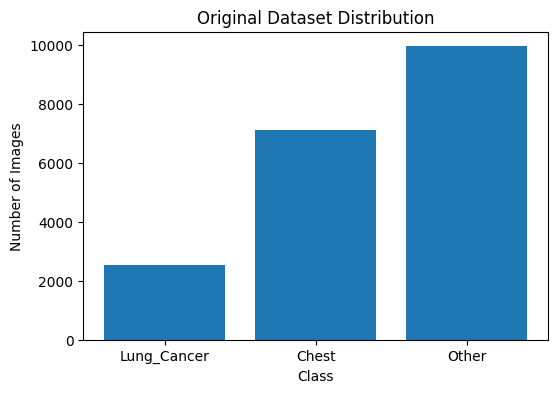
\includegraphics[
		width=\linewidth
		]{assets/dataset_dist_rm.png}
		
		\captionof{figure}{Distribution of the routing dataset classes.}
		\label{fig:routing_dataset_distribution}
		
	\end{minipage}
	
	\caption{Summary of the routing dataset distribution.}
	\label{fig:routing_dataset_summary}
\end{figure}

To ensure a fair evaluation procedure, the dataset was partitioned using a stratified sampling strategy. This approach preserved the original class distribution across all subsets and prevented sampling bias from influencing the evaluation results. The dataset was divided into training, validation, and testing subsets using a ratio of 70\%, 15\%, and 15\%, respectively.

A number of techniques were employed to mitigate the effects of class imbalance. First, class weights were incorporated during training to increase the contribution of minority classes to the optimization process. Second, stratified sampling was utilized to preserve representative class distributions across all dataset splits. Third, extensive data augmentation was applied to improve generalization and increase sample diversity. The augmentation pipeline included common image transformation techniques such as rotation, translation, zooming, flipping, brightness adjustment, and contrast variation. Geometric transformations that could significantly distort medical structures, such as excessive shearing, were intentionally avoided in order to preserve clinically relevant image features.

All models were trained using a batch size of 8 for a total of 10 epochs. The same training, validation, and testing partitions were used across all experiments to ensure consistency when comparing model performance.

\subsection{Learning Rate Optimization}

Since learning rate selection plays a crucial role in determining convergence behavior and final model performance, multiple learning rate values were investigated for each architecture. The evaluated learning rates included \(10^{-5}\), \(10^{-4}\), \(10^{-3}\), and \(10^{-2}\).

The experiments revealed that different architectures exhibited different optimization characteristics. DenseNet121 and ResNet50 achieved their highest performance when trained using a learning rate of \(10^{-2}\), whereas EfficientNetB3 performed best with a learning rate of \(10^{-4}\). Due to its relatively shallow architecture and limited feature extraction capacity, the custom convolutional neural network achieved its best results with a learning rate of \(10^{-5}\).

Table~\ref{tab:learning_rates} summarizes the optimal learning rate selected for each evaluated architecture.

\begin{table}[H]
	\centering
	\caption{Optimal learning rates identified during hyperparameter tuning.}
	\label{tab:learning_rates}
	\begin{tabular}{|l|c|}
		\hline
		\textbf{Model} & \textbf{Optimal Learning Rate} \\
		\hline
		Custom CNN & $10^{-5}$ \\
		\hline
		ResNet50 & $10^{-2}$ \\
		\hline
		DenseNet121 & $10^{-2}$ \\
		\hline
		EfficientNetB3 & $10^{-4}$ \\
		\hline
	\end{tabular}
\end{table}

These findings highlight the importance of architecture-specific hyperparameter tuning. Applying a common learning rate across all models would have resulted in suboptimal performance and potentially misleading comparisons between candidate architectures.

\subsection{Comparative Evaluation of Candidate Architectures}

To identify the most suitable backbone architecture for the routing model, four candidate architectures were trained and evaluated under identical conditions. The evaluated architectures included a custom CNN developed specifically for this task, ResNet50, DenseNet121, and EfficientNetB3.

The comparison focused on commonly used classification metrics, including accuracy, precision, recall, F1-score, and loss. Table~\ref{tab:routing_model_comparison} summarizes the performance of all evaluated architectures.

\begin{table}[H]
	\centering
	\caption{Performance comparison of candidate routing architectures.}
	\label{tab:routing_model_comparison}
	\begin{tabular}{|l|c|c|c|c|c|}
		\hline
		\textbf{Model} &
		\textbf{Accuracy} &
		\textbf{Precision} &
		\textbf{Recall} &
		\textbf{F1-Score} &
		\textbf{Loss} \\
		\hline
		Custom CNN & 1.0000 & 1.0000 & 1.0000 & 1.0000 & 0.0011 \\
		\hline
		ResNet50 & 1.0000 & 1.0000 & 1.0000 & 1.0000 & $1.782 \times 10^{-6}$ \\
		\hline
		EfficientNetB3 & 1.0000 & 1.0000 & 1.0000 & 1.0000 & $1.9816 \times 10^{-5}$ \\
		\hline
		DenseNet121 & 1.0000 & 1.0000 & 1.0000 & 1.0000 & $1.5126 \times 10^{-7}$ \\
		\hline
	\end{tabular}
\end{table}

The results demonstrate the superiority of DenseNet121 for the routing task. DenseNet121 achieved perfect classification performance on the test dataset, obtaining an accuracy, precision, recall, and F1-score of 100\%. Furthermore, the model achieved an extremely low loss value of \(1.5126 \times 10^{-7}\), indicating highly confident predictions and excellent convergence behavior.

The dense connectivity mechanism employed by DenseNet121 enables efficient feature reuse throughout the network and facilitates gradient propagation across deep layers. As a result, the model was able to learn highly discriminative representations that effectively separated the three image categories. Based on these findings, DenseNet121 was selected as the backbone architecture of the final routing model.

\begin{figure}[htbp]
	\centering
	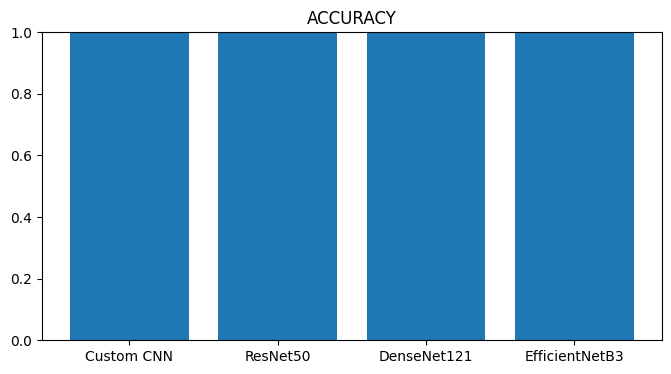
\includegraphics[width=\linewidth]{assets/models_acc_rm.png}
	\caption{Comparison of classification accuracy across all evaluated routing architectures.}
	\label{fig:routing_accuracy_comparison}
\end{figure}

\subsection{Training and Validation Behavior}

In addition to evaluating final classification performance, the training dynamics of each architecture were analyzed to assess convergence behavior and learning stability throughout the optimization process.

Figures~\ref{fig:routing_training_curves} illustrate the evolution of training accuracy, validation accuracy, training loss, and validation loss during the training process for all evaluated models.

\begin{figure}[htbp]
	\centering
	
	% -------------------------------------------------
	% Custom CNN
	% -------------------------------------------------
	\begin{subfigure}{0.95\textwidth}
		\centering
		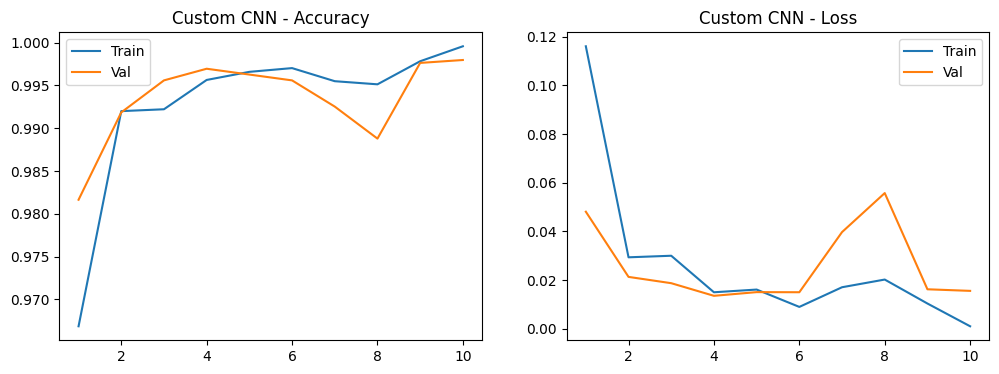
\includegraphics[
		width=\linewidth,
		height=0.18\textheight,
		keepaspectratio
		]{assets/curve_customcnn.png}
		\caption{Training and validation curves for the Custom CNN model.}
		\label{fig:customcnn_training_curves}
	\end{subfigure}
	
	\vspace{0.25cm}
	
	% -------------------------------------------------
	% ResNet50
	% -------------------------------------------------
	\begin{subfigure}{0.95\textwidth}
		\centering
		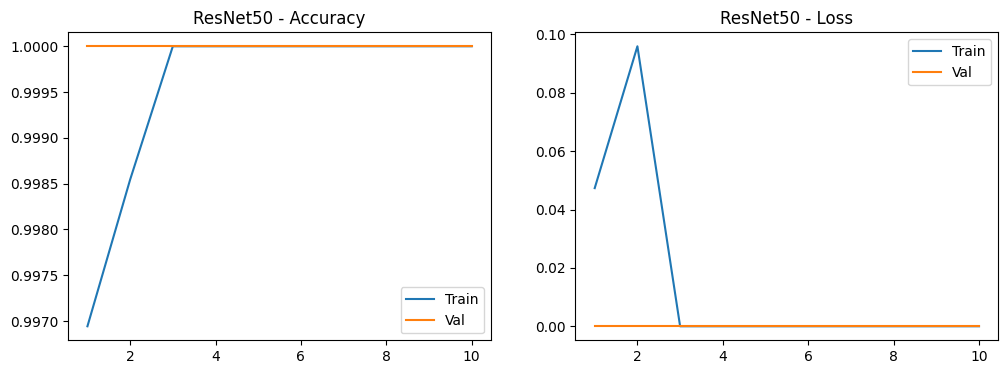
\includegraphics[
		width=\linewidth,
		height=0.18\textheight,
		keepaspectratio
		]{assets/curve_resnet.png}
		\caption{Training and validation curves for the ResNet50 model.}
		\label{fig:resnet50_training_curves}
	\end{subfigure}
	
	\vspace{0.25cm}
	
	% -------------------------------------------------
	% EfficientNetB3
	% -------------------------------------------------
	\begin{subfigure}{0.95\textwidth}
		\centering
		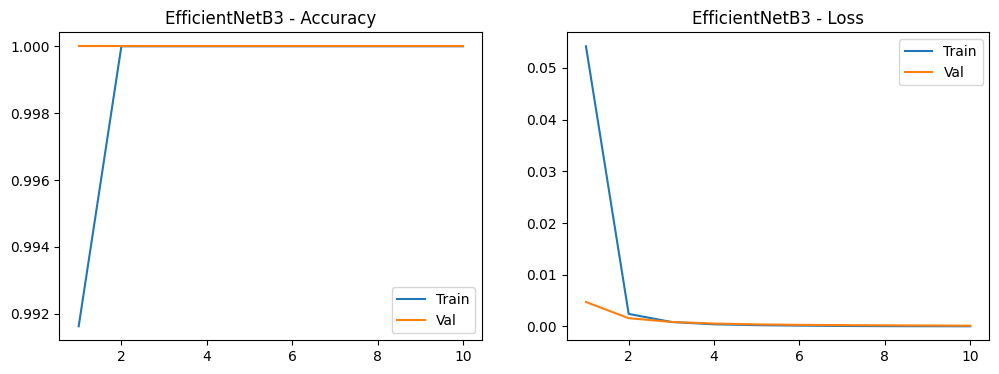
\includegraphics[
		width=\linewidth,
		height=0.18\textheight,
		keepaspectratio
		]{assets/curve_efficient.png}
		\caption{Training and validation curves for the EfficientNetB3 model.}
		\label{fig:efficientnet_training_curves}
	\end{subfigure}
	
	\vspace{0.25cm}
	
	% -------------------------------------------------
	% DenseNet121
	% -------------------------------------------------
	\begin{subfigure}{0.95\textwidth}
		\centering
		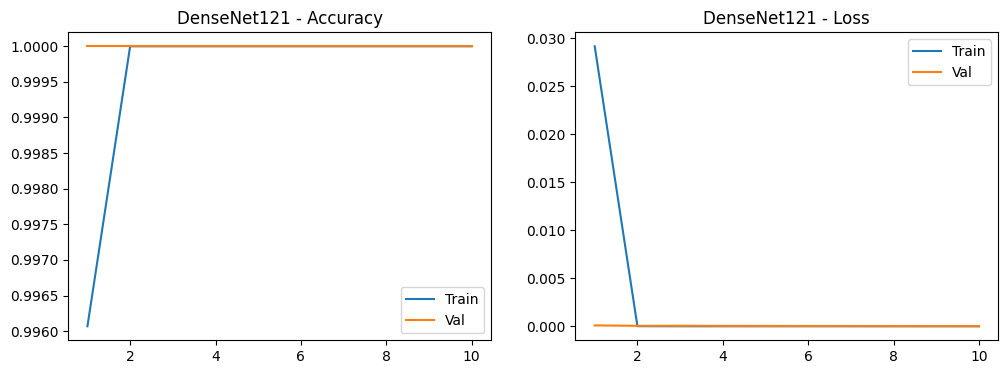
\includegraphics[
		width=\linewidth,
		height=0.18\textheight,
		keepaspectratio
		]{assets/curve_densenet.png}
		\caption{Training and validation curves for the DenseNet121 model.}
		\label{fig:densenet121_training_curves}
	\end{subfigure}
	
	\caption{Training and validation performance curves for all evaluated routing model architectures. Each figure illustrates the evolution of accuracy and loss throughout the training process and provides insight into model convergence, optimization stability, and generalization behavior.}
	\label{fig:routing_training_curves}
\end{figure}

Analysis of these curves provides valuable insight into convergence speed, optimization stability, and generalization behavior. The results indicate that DenseNet121 exhibited rapid convergence while maintaining stable validation performance throughout training, further supporting its selection as the final routing architecture.

\subsection{Confusion Matrix Analysis}

To further investigate classification performance, confusion matrices were generated for each evaluated architecture. Confusion matrices provide a detailed view of model predictions by illustrating the relationship between true class labels and predicted class labels.

The confusion matrix analysis is particularly important for the routing stage because misclassification at this level may cause images to be forwarded to an inappropriate downstream diagnostic model. Therefore, minimizing routing errors is essential for ensuring the reliability of the entire hierarchical framework.

Figure~\ref{fig:all_confusion_matrices} presents the confusion matrices obtained for all evaluated architectures.

\begin{figure}[htbp]
	\centering
	
	% ---------------- Row 1 ----------------
	\begin{subfigure}[t]{0.48\textwidth}
		\centering
		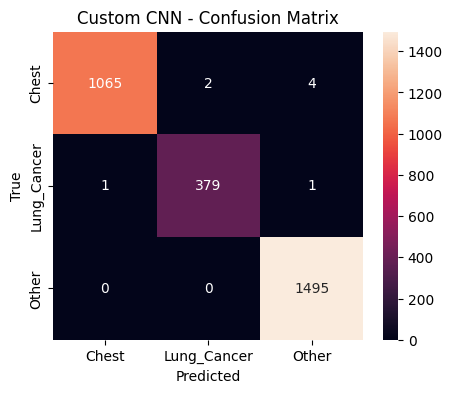
\includegraphics[
		width=\linewidth,
		height=0.28\textheight,
		keepaspectratio
		]{assets/customcnn_cm_rm.png}
		\caption{Custom CNN}
	\end{subfigure}
	\hfill
	\begin{subfigure}[t]{0.48\textwidth}
		\centering
		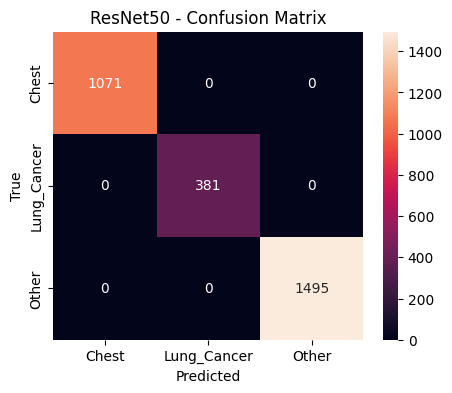
\includegraphics[
		width=\linewidth,
		height=0.28\textheight,
		keepaspectratio
		]{assets/resnet50_cm_rm.png}
		\caption{ResNet50}
	\end{subfigure}
	
	\vspace{0.3cm}
	
	% ---------------- Row 2 ----------------
	\begin{subfigure}[t]{0.48\textwidth}
		\centering
		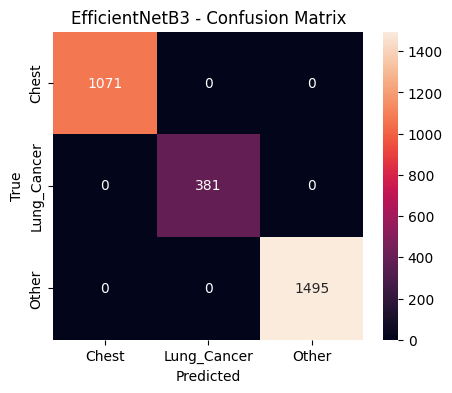
\includegraphics[
		width=\linewidth,
		height=0.28\textheight,
		keepaspectratio
		]{assets/efficient_cm_rm.png}
		\caption{EfficientNetB3}
	\end{subfigure}
	\hfill
	\begin{subfigure}[t]{0.48\textwidth}
		\centering
		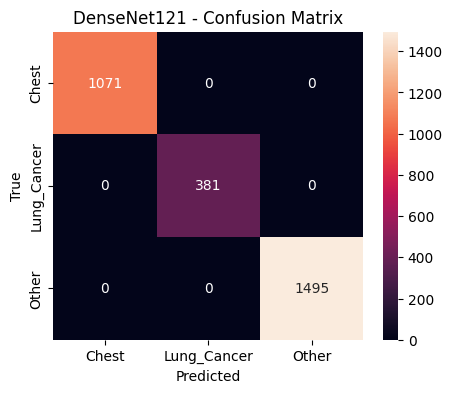
\includegraphics[
		width=\linewidth,
		height=0.28\textheight,
		keepaspectratio
		]{assets/densenet_cm_rm.png}
		\caption{DenseNet121}
	\end{subfigure}
	
	\caption{Confusion matrices for all evaluated routing models across the three classes.}
	\label{fig:all_confusion_matrices}
\end{figure}

The confusion matrix corresponding to DenseNet121 demonstrated perfect classification performance across all three classes, with no observed misclassifications in the test set. This result confirms the model's ability to accurately distinguish between chest X-ray images, chest CT scans, and out-of-distribution images, making it highly suitable for deployment as the first-level routing component within the proposed framework.

\subsection{Discussion}

The experimental results demonstrate that the proposed routing model successfully fulfills its intended objective of accurately identifying image modalities and directing images toward the appropriate diagnostic pathway. The combination of transfer learning, data augmentation, class weighting, and hyperparameter optimization enabled the evaluated architectures to achieve strong classification performance despite the inherent challenges associated with heterogeneous medical imaging data.

Among all tested architectures, DenseNet121 consistently produced the most favorable results and achieved perfect performance on the test dataset. The model's dense connectivity structure enabled efficient feature reuse and facilitated the extraction of highly discriminative modality-specific representations. Furthermore, the confusion matrix analysis confirmed the absence of routing errors, indicating that all images were successfully assigned to their correct categories.

These findings validate the effectiveness of the proposed first-level routing strategy and demonstrate that the routing component provides a reliable foundation for the subsequent disease classification and lung cancer detection stages of the overall framework.

% Relax float placement constraints for this section to improve page utilization
\renewcommand{\topfraction}{.85}
\renewcommand{\bottomfraction}{.7}
\renewcommand{\textfraction}{.15}
\renewcommand{\floatpagefraction}{.66}
\setcounter{topnumber}{9}
\setcounter{bottomnumber}{9}
\setcounter{totalnumber}{20}

\section{Chest Disease Classification Experiments}

This section documents the experimental results obtained from the evaluation of various deep learning architectures for chest disease classification. Both centralized and federated learning paradigms are explored to assess performance, generalization, and privacy-preserving capabilities.

\subsection{Implementation Environment and Development Tools}

This section documents the hardware infrastructure, software environment, and development frameworks employed throughout the experimental evaluation of the proposed chest disease classification system. Reproducibility of results depends critically on the precise specification of the computational environment, and accordingly all relevant configurations are reported below.

\subsubsection{Hardware Environment}

All centralized training experiments (preprocessing, U-Net segmentation, DenseNet121, ResNet50V2, EfficientNet, and VGG-19 classification models) were conducted on a cloud-based GPU accelerated computational environment. The hardware specifications and computed class weights are summarized in Table~\ref{tab:chest_hardware} and Table~\ref{tab:chest_computed_weights}, respectively.

{\renewcommand{\arraystretch}{1.2}
\begin{table}[htbp]
    \centering
    \begin{minipage}[c]{0.52\textwidth}
        \centering
        \caption{Hardware specifications.}
        \label{tab:chest_hardware}
        \small
        \begin{tabularx}{\textwidth}{|l|X|}
            \hline
            \textbf{Component} & \textbf{Specification} \\
            \hline
            Compute Platform & Colab Pro \\
            \hline
            GPU & NVIDIA T4 (15 GB) \\
            \hline
            CPU & Intel Xeon (2 vCPUs) \\
            \hline
            System RAM & 12--51 GB \\
            \hline
            Storage & Google Drive \\
            \hline
            OS & Ubuntu 20.04 LTS \\
            \hline
        \end{tabularx}
    \end{minipage}
    \hfill
    \begin{minipage}[c]{0.44\textwidth}
        \centering
        \caption{Computed class weights.}
        \label{tab:chest_computed_weights}
        \small
        \begin{tabularx}{\textwidth}{|l|c|X|}
            \hline
            \textbf{Class} & $N_k$ & \textbf{Weight $w_k$} \\
            \hline
            Normal & 4,870 & $\sim$0.78 \\
            \hline
            Pneu. & 4,221 & $\sim$0.90 \\
            \hline
            COVID & 3,192 & $\sim$1.19 \\
            \hline
            TB & 2,946 & $\sim$1.29 \\
            \hline
        \end{tabularx}
    \end{minipage}
\end{table}
}

The Federated Learning simulation experiments required more intensive multi-process resource management due to the Ray-based client parallelism used by the Flower framework. Resources were allocated per client using Ray's resource reservation mechanism, as detailed in Section~\ref{sec:federated_results}.

\subsubsection{Software Frameworks and Libraries}

The implementation stack is summarized in Table~\ref{tab:chest_software}. All dependencies were installed within the Colab environment, with version pinning applied where reproducibility was critical.

\begin{table}[htbp]
	\centering
	\caption{Software framework and library stack.}
	\label{tab:chest_software}
	\small
	\begin{tabularx}{\textwidth}{|l|l|X|}
		\hline
		\textbf{Library / Framework} & \textbf{Version / Source} & \textbf{Purpose} \\
		\hline
		Python & 3.10 & Primary programming language \\
		\hline
		TensorFlow / Keras & 2.15.1 & Centralized model training (U-Net, DenseNet, ResNet, EfficientNet, VGG) \\
		\hline
		PyTorch & 2.1.0 & Federated Learning model backbone (DenseNet121) \\
		\hline
		Torchvision & 0.16.1 & Pre-trained model weights, image transforms \\
		\hline
		Flower (flwr) & 1.4 (simulation) & Federated Learning framework (FedAvg strategy) \\
		\hline
		Ray & 2.1 & Distributed simulation backend for Flower \\
		\hline
		OpenCV (cv2) & 4.8.2 & Image preprocessing (CLAHE, Gaussian blur, normalization) \\
		\hline
		NumPy & 1.24.0 & Numerical computation \\
		\hline
		Scikit-learn & 1.3.0 & Classification reports, confusion matrices, AUC computation \\
		\hline
		Matplotlib & 3.7.1 & Training history plots, visualization \\
		\hline
		tqdm & 4.66.1 & Training progress bars \\
		\hline
		Pandas & 2.0.2 & Misclassification analysis and CSV export \\
		\hline
	\end{tabularx}
\end{table}

\subsubsection{Development Workflow}

All experiments were developed iteratively in Jupyter Notebooks within the Google Colab environment, with datasets mounted from Google Drive. The local preprocessing pipeline (CLAHE, Gaussian blur, normalization) was executed on a local machine equipped with an NVIDIA GPU, and the resulting processed dataset was uploaded to Google Drive for cloud-based training. Model checkpoints, final weights, and evaluation artefacts were saved both locally and to Drive for persistence across Colab session resets.

Mixed precision training (float16 for computations, float32 for master weights) was enabled throughout using TensorFlow's Automatic Mixed Precision (AMP) for TensorFlow experiments, providing approximately 2--3$\times$ speed improvement on Tensor Core-equipped NVIDIA GPUs with negligible accuracy impact.

\subsection{Dataset Preparation and Experimental Setup}

\subsubsection{Dataset Splits and Class Distribution}

The full composite dataset of 17,637 images was partitioned into training, validation, and test sets. The training set (15,229 images) was used exclusively for gradient-based parameter updates. The validation set was used for early stopping, learning rate scheduling, and model selection. The test set was kept strictly held out throughout all training and validation activities and was accessed only once for final performance evaluation.

{\renewcommand{\arraystretch}{1.2}
\begin{table}[htbp]
    \centering
    \begin{minipage}[c]{0.52\textwidth}
        \centering
        \caption{Complete dataset split.}
        \label{tab:chest_dataset_splits}
        \small
        \begin{tabularx}{\textwidth}{|l|c|c|c|c|}
            \hline
            \textbf{Class} & \textbf{Train} & \textbf{Val} & \textbf{Test} & \textbf{Total} \\
            \hline
            Normal & 4,870 & $\sim$610 & $\sim$610 & $\sim$6,090 \\
            \hline
            Pneu. & 4,221 & $\sim$528 & $\sim$528 & $\sim$5,277 \\
            \hline
            COVID & 3,192 & $\sim$400 & $\sim$400 & $\sim$3,992 \\
            \hline
            TB & 2,946 & $\sim$368 & $\sim$368 & $\sim$3,682 \\
            \hline
            \textbf{Total} & \textbf{15,229} & \textbf{1,906} & \textbf{1,906} & \textbf{19,041} \\
            \hline
        \end{tabularx}
    \end{minipage}
    \hfill
    \begin{minipage}[c]{0.44\textwidth}
        \centering
        \caption{Data augmentation parameters.}
        \label{tab:chest_augmentation}
        \small
        \begin{tabularx}{\textwidth}{|l|l|X|}
            \hline
            \textbf{Aug.} & \textbf{Param.} & \textbf{Just.} \\
            \hline
            Rotation & $\pm$15$^\circ$ & Position \\
            \hline
            W-Shift & $\pm$10\% & Lat. Trans. \\
            \hline
            H-Shift & $\pm$10\% & C-C Var. \\
            \hline
            Zoom & $\pm$10\% & SID Var. \\
            \hline
            H-Flip & $p=0.5$ & Symmetry \\
            \hline
            Fill & Zero & Textures \\
            \hline
        \end{tabularx}
    \end{minipage}
\end{table}
}

\textbf{Note on Class Imbalance:} The training set exhibits a moderate class imbalance, with Normal (32\%) substantially over-represented relative to Tuberculosis (19.3\%). Inverse-frequency class weights are applied during training for all models to counteract this imbalance and prevent the classifier from developing a bias toward more frequent classes.

\subsubsection{Data Augmentation Strategy}

Online data augmentation is applied exclusively to the training set using Keras's \texttt{ImageDataGenerator} API (for TensorFlow experiments) and \texttt{torchvision.transforms} (for Federated Learning experiments). The augmentation policy was carefully selected to apply only transformations that are plausible within the domain of chest radiography --- preserving diagnostic realism while increasing data diversity.

Notably, vertical flipping and brightness/contrast jitter are excluded to preserve diagnostic realism and avoid conflict with CLAHE preprocessing. Augmentations are applied only at training time; validation and test generators apply only the rescaling operation.

\subsubsection{Class Weighting}

To further address class imbalance beyond augmentation, inverse-frequency class weights are computed from the training set label distribution and passed to the model's \texttt{fit()} call. For each class $k$:
\begin{equation}
	w_k = \frac{N_{\text{total}}}{K \cdot N_k}
	\label{eq:chest_weights}
\end{equation}
where $K=4$, $N_{\text{total}}=15,229$, and $N_k$ is the number of training samples of class $k$. The computed weights for the training set are summarized in Table~\ref{tab:chest_computed_weights}.

\subsubsection{Evaluation Metrics}

Model performance is evaluated using a comprehensive set of metrics reflecting both overall and class-specific diagnostic performance:
\begin{itemize}
    \item \textbf{Accuracy:} $\frac{TP+TN}{TP+TN+FP+FN}$ --- overall proportion of correct predictions.
    \item \textbf{Precision (Positive Predictive Value):} $\frac{TP}{TP+FP}$ --- fraction of positive predictions that are correct.
    \item \textbf{Recall (Sensitivity):} $\frac{TP}{TP+FN}$ --- fraction of true positives correctly detected.
    \item \textbf{F1-Score:} $2 \cdot \frac{\text{Precision} \cdot \text{Recall}}{\text{Precision} + \text{Recall}}$ --- harmonic mean of precision and recall.
    \item \textbf{AUC-ROC:} Area under the Receiver Operating Characteristic curve (for OVR models, evaluated per class and macro-averaged).
    \item \textbf{Confusion Matrix:} A matrix showing the breakdown of correct and incorrect predictions across all class pairs.
\end{itemize}

\subsection{Segmentation Training Results}

The segmentation model was trained on a dataset of 6,106 annotated images, with an 85:15 split between training and validation sets. Early stopping was applied, terminating training at epoch 15 out of a maximum of 50 epochs. The model was optimized using the Adam optimizer with a learning rate of $10^{-4}$ and a combined Binary Cross-Entropy (BCE) and Dice loss function.

\begin{table}[h]
	\centering
	\caption{Segmentation Model Performance on the Validation Set}
	\label{tab:segmentation_results}
	\begin{tabular}{lc}
		\hline
		\textbf{Metric} & \textbf{Value} \\
		\hline
		Validation Accuracy & 95.86\% \\
		Training Accuracy & 98.14\% \\
		Validation Loss & 0.0904 \\
		Dice Coefficient & 0.9592 \\
		IoU Score & 0.9756 \\
		\hline
	\end{tabular}
\end{table}

The obtained results demonstrate excellent segmentation performance. The model achieved a validation accuracy of 95.86\% with a low validation loss of 0.0904, indicating good generalization capability. Furthermore, the Dice coefficient of 0.9592 and IoU score of 0.9756 confirm a high degree of overlap between the predicted masks and the ground-truth annotations, highlighting the effectiveness of the proposed segmentation approach.

\subsection{Single-Label Classification Results (SoftMax Approach)}

The SoftMax approach treats the four-class chest disease classification as a standard single-label multi-class problem: each image is assigned exactly one diagnostic class, and the output layer applies the SoftMax function to produce a valid probability distribution over the four classes:
\begin{equation}
	\hat{y}_k = \frac{e^{z_k}}{\sum_{j=1}^K e^{z_j}}, \quad \sum_{k=1}^K \hat{y}_k = 1
\end{equation}
The predicted class is $\hat{k} = \arg\max_k \hat{y}_k$, and the loss function is sparse categorical cross-entropy:
\begin{equation}
	\mathcal{L}_{\text{CE}} = -\log \hat{y}_{y_{\text{true}}}
\end{equation}

\subsubsection{DenseNet121 (SoftMax, Two-Phase Fine-Tuning)}

The first evaluated architecture is DenseNet121 with SoftMax output, trained using a two-phase fine-tuning strategy designed to maximize the transfer learning benefit while progressively adapting the network to the chest disease classification task. Key hyperparameters are detailed in Table~\ref{tab:densenet_softmax_params}. The learning curves, confusion matrix, and classification report for this model are shown in Figure~\ref{fig:densenet_softmax_curves}, Figure~\ref{fig:densenet_softmax_cm}, and Figure~\ref{fig:densenet_softmax_report}, respectively.

\textbf{Phase 1 --- Feature Extraction:} The DenseNet121 base is initialized with ImageNet weights. The last 100 layers are made trainable while all preceding layers are frozen. This selective unfreezing ensures that the early-stage feature extractors (which learn generic low-level features such as edges and textures --- applicable across domains) are preserved, while the deeper, task-specific layers are fine-tuned for chest pathology discrimination. The custom classification head (GAP $\to$ BN $\to$ Dense(512) $\to$ Dropout(0.4) $\to$ Dense(256) $\to$ Dropout(0.3) $\to$ Dense(4, SoftMax)) is trained end-to-end for a maximum of 40 epochs with the Adam optimizer at an initial learning rate of $10^{-4}$.

\textbf{Phase 2 --- Deep Fine-Tuning:} The best Phase 1 checkpoint is loaded, and the trainable scope is extended to the last 200 layers of the DenseNet121 base. The learning rate is significantly reduced to $10^{-6}$ (100$\times$ smaller) to ensure that the pre-trained weights are refined gently rather than disrupted. A maximum of 10 additional epochs are run. This two-phase strategy prevents the "catastrophic forgetting" of ImageNet representations that can occur when fine-tuning with an aggressive learning rate.

{\renewcommand{\arraystretch}{1.2}
\begin{table}[htbp]
	\centering
	\caption{DenseNet121 SoftMax --- Key Hyperparameters.}
	\label{tab:densenet_softmax_params}
	\small
	\begin{tabularx}{0.9\textwidth}{|X|l|l|}
		\hline
		\textbf{Parameter} & \textbf{Phase 1} & \textbf{Phase 2} \\
		\hline
		Trainable layers & Last 100 & Last 200 \\
		\hline
		Optimizer & Adam & Adam \\
		\hline
		Learning rate & $10^{-4}$ & $10^{-6}$ \\
		\hline
		Max epochs & 40 & 10 \\
		\hline
		Loss & \multicolumn{2}{l|}{Sparse Categorical Cross-Entropy} \\
		\hline
		Batch size & 32 & 32 \\
		\hline
		Early stopping & \multicolumn{2}{l|}{patience=8, monitor=val\_accuracy} \\
		\hline
		LR reduction & \multicolumn{2}{l|}{ReduceLROnPlateau (factor=0.2, patience=3)} \\
		\hline
	\end{tabularx}
\end{table}
}

\begin{figure}[htbp]
	\centering
	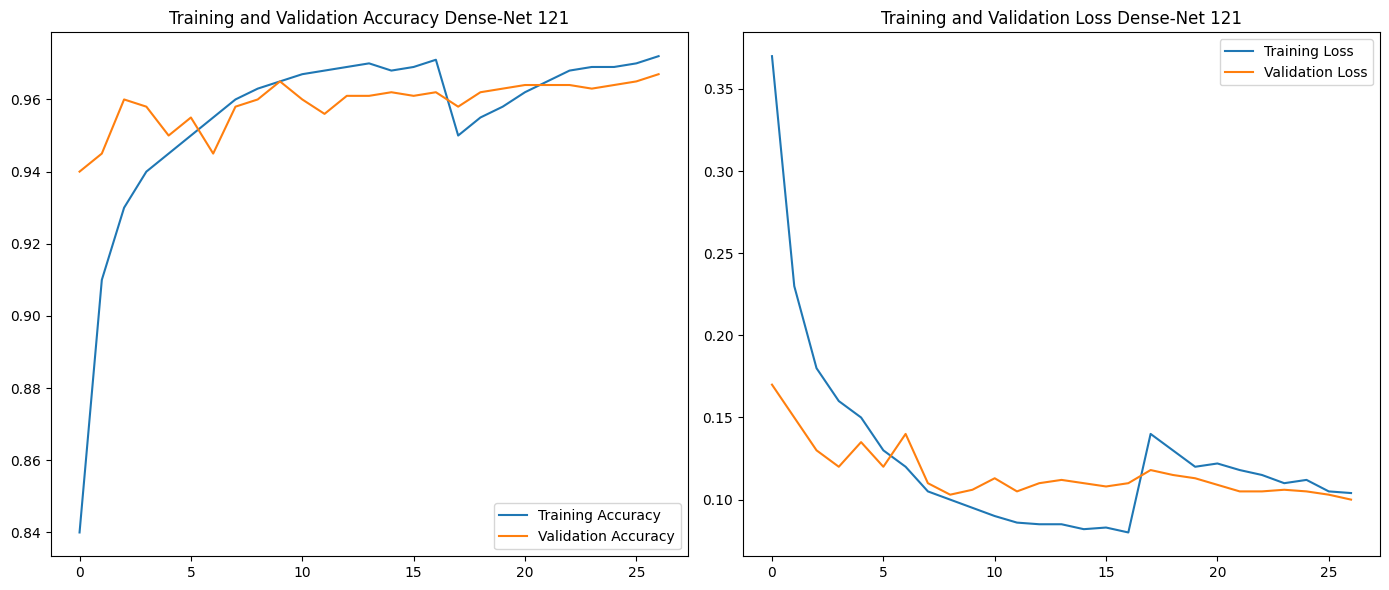
\includegraphics[width=0.85\textwidth, height=7cm, keepaspectratio]{assets/chest_model/image1.png}
	\caption{Learning curves for DenseNet121 SoftMax.}
	\label{fig:densenet_softmax_curves}
\end{figure}

\begin{figure}[htbp]
	\centering
	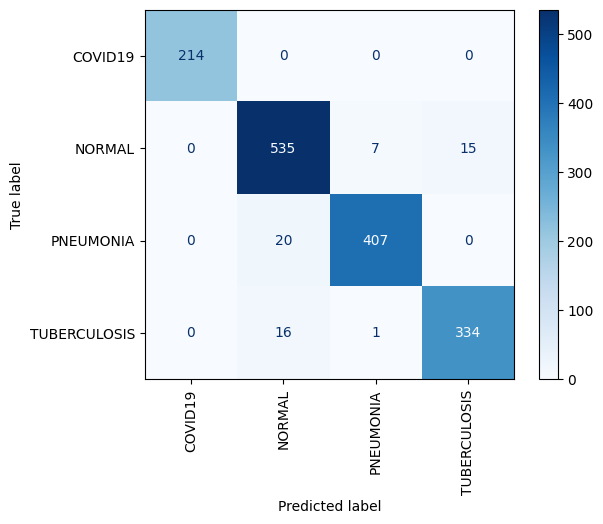
\includegraphics[width=0.7\textwidth, height=8cm, keepaspectratio]{assets/chest_model/image2.png}
	\caption{Confusion matrix for DenseNet121 SoftMax.}
	\label{fig:densenet_softmax_cm}
\end{figure}

\begin{figure}[htbp]
	\centering
	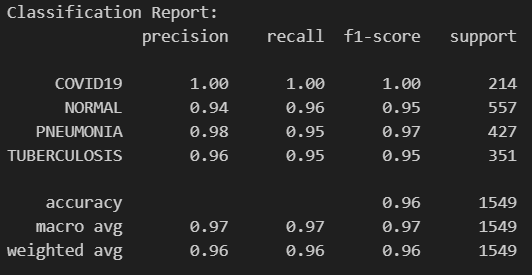
\includegraphics[width=0.85\textwidth, height=9cm, keepaspectratio]{assets/chest_model/image3.png}
	\caption{Classification report for DenseNet121 SoftMax.}
	\label{fig:densenet_softmax_report}
\end{figure}

\subsubsection{ResNet50V2 (Softmax, Partial Fine-Tuning)}

The second SoftMax baseline employs ResNet50V2 (He et al., 2016, V2 with pre-activation residual blocks), a 50-layer residual network pre-trained on ImageNet. ResNet50V2 introduces significant architectural improvements over the original ResNet50, including full pre-activation order (BN $\to$ ReLU $\to$ Conv rather than Conv $\to$ BN $\to$ ReLU), which leads to improved gradient flow and training stability. The model follows a partial fine-tuning strategy in which the last 40 layers are unfrozen for task-specific adaptation while the earlier layers retain their ImageNet representations.

The classification head follows the same structural template as DenseNet121: GAP $\to$ Dense(512, ReLU) $\to$ Dropout(0.4) $\to$ Dense(256, ReLU) $\to$ Dense(4, SoftMax). A notably lower learning rate of $10^{-4}$ is used from the outset, reflecting the more conservative fine-tuning approach appropriate for ResNet50V2's architecture. Key hyperparameters are listed in Table~\ref{tab:resnet_softmax_params}, with experimental results shown in Figure~\ref{fig:resnet_softmax_curves}, Figure~\ref{fig:resnet_softmax_cm}, and Figure~\ref{fig:resnet_softmax_report}. Training runs for a maximum of 30 epochs with early stopping (patience=7).

{\renewcommand{\arraystretch}{1.2}
\begin{table}[htbp]
	\centering
	\caption{ResNet50V2 SoftMax --- Key Hyperparameters.}
	\label{tab:resnet_softmax_params}
	\small
	\begin{tabularx}{0.85\textwidth}{|X|l|}
		\hline
		\textbf{Parameter} & \textbf{Value} \\
		\hline
		Base architecture & ResNet50V2 (ImageNet pre-trained) \\
		\hline
		Trainable layers & Last 40 layers + head \\
		\hline
		Frozen layers & First $\sim$145 layers \\
		\hline
		Optimizer & Adam ($10^{-4}$) \\
		\hline
		Max epochs & 30 \\
		\hline
		Loss & Sparse Categorical Cross-Entropy \\
		\hline
		Batch size & 32 \\
		\hline
		Early stopping & patience=7, monitor=val\_accuracy \\
		\hline
		LR reduction & ReduceLROnPlateau (factor=0.2, patience=3) \\
		\hline
	\end{tabularx}
\end{table}
}

\begin{figure}[htbp]
	\centering
	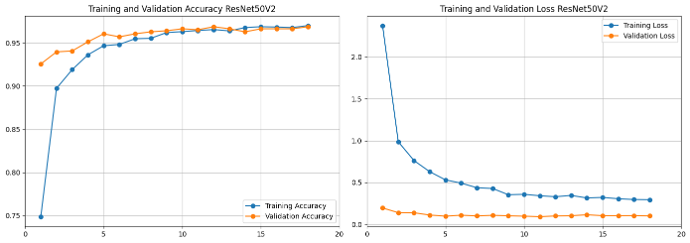
\includegraphics[width=\textwidth]{assets/chest_model/resnet-graphs.png}
	\caption{Learning curves for ResNet50V2 SoftMax.}
	\label{fig:resnet_softmax_curves}
\end{figure}

\begin{figure}[htbp]
	\centering
	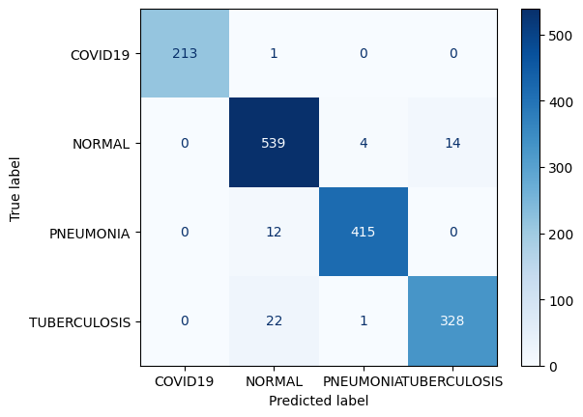
\includegraphics[width=\textwidth]{assets/chest_model/resnet-cm.png}
	\caption{Confusion matrix for ResNet50V2 SoftMax.}
	\label{fig:resnet_softmax_cm}
\end{figure}

\begin{figure}[htbp]
	\centering
	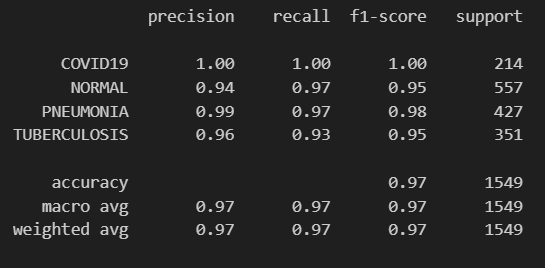
\includegraphics[width=0.85\textwidth, height=9cm, keepaspectratio]{assets/chest_model/image6.png}
	\caption{Classification report for ResNet50V2 SoftMax.}
	\label{fig:resnet_softmax_report}
\end{figure}

\FloatBarrier

\subsubsection{EfficientNet (SoftMax)}

EfficientNet scales network depth, width, and resolution jointly using a compound scaling coefficient, achieving state-of-the-art accuracy with fewer parameters than comparable architectures. The same classification head structure and training strategy are applied. Hyperparameters and results for EfficientNet are provided in Table~\ref{tab:efficientnet_softmax_params}, Figure~\ref{fig:efficientnet_softmax_curves}, Figure~\ref{fig:efficientnet_softmax_cm}, and Figure~\ref{fig:efficientnet_softmax_report}.

{\renewcommand{\arraystretch}{1.2}
\begin{table}[htbp]
	\centering
	\caption{EfficientNet SoftMax --- Key Hyperparameters.}
	\label{tab:efficientnet_softmax_params}
	\small
	\begin{tabularx}{0.85\textwidth}{|X|l|}
		\hline
		\textbf{Parameter} & \textbf{Value} \\
		\hline
		Base architecture & EfficientNetB0 (ImageNet pre-trained) \\
		\hline
		Trainable layers & Last 200 layers \\
		\hline
		Optimizer & Adam ($10^{-4}$) \\
		\hline
		Max epochs & 30 \\
		\hline
		Loss & Sparse Categorical Cross-Entropy \\
		\hline
		Batch size & 32 \\
		\hline
		Early stopping & patience=7, monitor=val\_accuracy \\
		\hline
		LR reduction & ReduceLROnPlateau (factor=0.2, patience=3) \\
		\hline
	\end{tabularx}
\end{table}
}

\begin{figure}[htbp]
	\centering
	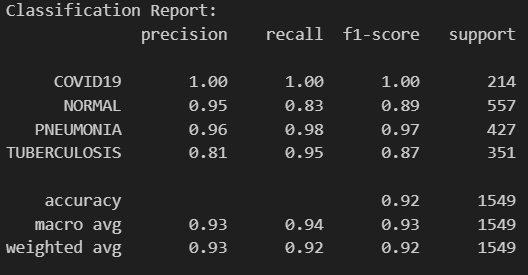
\includegraphics[width=0.85\textwidth, height=7cm, keepaspectratio]{assets/chest_model/image9.png}
	\caption{Classification report for EfficientNet SoftMax.}
	\label{fig:efficientnet_softmax_report}
\end{figure}

\begin{figure}[htbp]
	\centering
	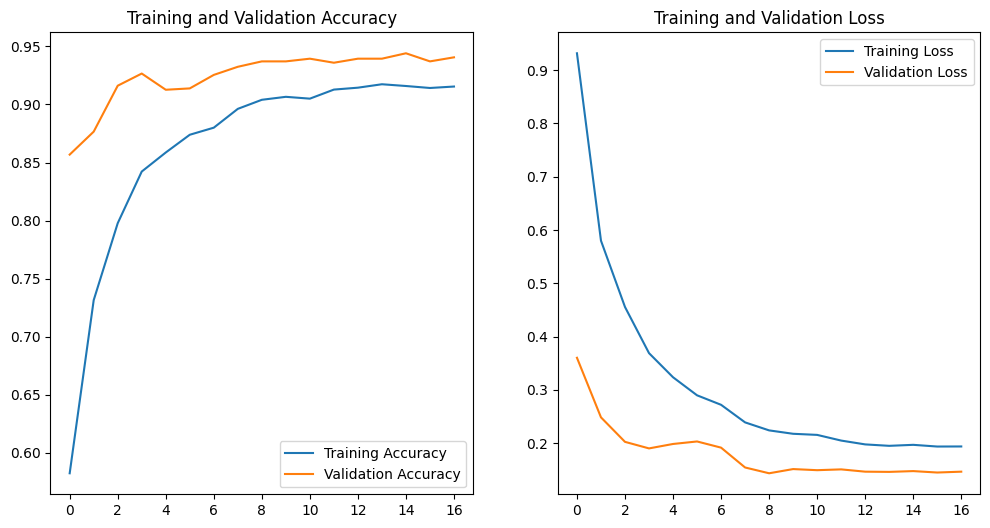
\includegraphics[width=\textwidth]{assets/chest_model/image7.png}
	\caption{Learning Curves for EfficientNet SoftMax.}
	\label{fig:efficientnet_softmax_curves}
\end{figure}

\begin{figure}[htbp]
	\centering
	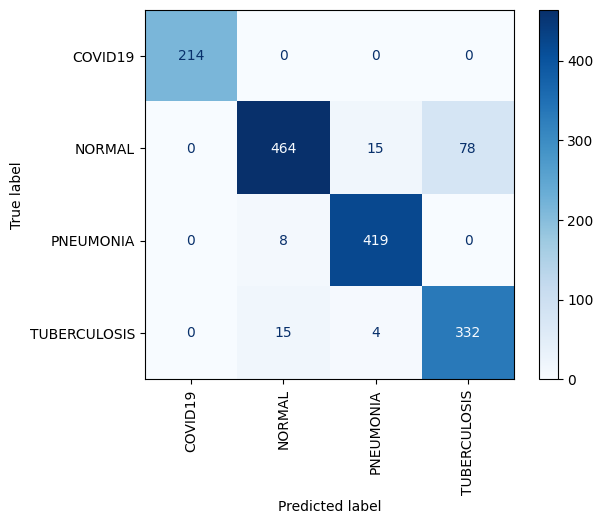
\includegraphics[width=\textwidth]{assets/chest_model/image8.png}
	\caption{Confusion matrix for EfficientNet SoftMax.}
	\label{fig:efficientnet_softmax_cm}
\end{figure}

\FloatBarrier

\subsubsection{VGG-19 (SoftMax)}

VGG-19 is a deep convolutional network with 19 weight layers characterized by a uniform architecture of convolutions and max-pooling operations. Despite its comparatively large parameter count, it remains a strong baseline for medical image classification due to its simple and well-understood feature hierarchy. Hyperparameters for VGG-19 are summarized in Table~\ref{tab:vgg_softmax_params}.

{\renewcommand{\arraystretch}{1.2}
\begin{table}[htbp]
	\centering
	\caption{VGG-19 SoftMax --- Key Hyperparameters.}
	\label{tab:vgg_softmax_params}
	\small
	\begin{tabularx}{0.85\textwidth}{|X|l|}
		\hline
		\textbf{Parameter} & \textbf{Value} \\
		\hline
		Base architecture & VGG-19 (ImageNet pre-trained) \\
		\hline
		Trainable layers & Last 5 conv layers + head \\
		\hline
		Optimizer & Adam ($10^{-5}$) \\
		\hline
		Max epochs & 30 \\
		\hline
		Loss & Sparse Categorical Cross-Entropy \\
		\hline
		Batch size & 32 \\
		\hline
		Early stopping & patience=7, monitor=val\_accuracy \\
		\hline
		LR reduction & ReduceLROnPlateau (factor=0.2, patience=3) \\
		\hline
	\end{tabularx}
\end{table}
}

Table~\ref{tab:vgg_res} presents the results achieved by the VGG-19 model configured with a Softmax activation function for multi-class chest disease classification. Overall, the model demonstrates strong discriminative capability across the four target classes (COVID-19, Normal, Pneumonia, and Tuberculosis), benefiting from the deep hierarchical feature extraction of the VGG-19 architecture. However, compared to more recent architectures, a slight reduction in generalization performance can be observed, particularly in visually similar classes such as Pneumonia and Tuberculosis, which often share overlapping radiographic patterns and therefore present a more challenging classification boundary.

The training dynamics of the model were recorded during training and are illustrated in Figure~\ref{fig:vgg_curves}, showing a generally stable convergence with steadily improving training and validation accuracy across epochs. A small generalization gap emerges in later epochs, indicating mild overfitting typical of high-capacity CNNs trained on limited medical datasets. The confusion matrix in Figure~\ref{fig:vgg-cm} further details class-wise prediction behavior, highlighting that most misclassifications occur between Pneumonia and Tuberculosis due to their radiographic similarity, while COVID-19 samples are classified more consistently due to more distinctive visual patterns. In addition, the final classification report shown in Figure~\ref{fig:vgg-report} confirms strong precision, recall, and F1-scores across most classes, providing a comprehensive evaluation of the model’s diagnostic performance.

\begin{table}[H]
	\centering
	\caption{Training Configuration and Performance Summary}
	\label{tab:vgg_res}
	\renewcommand{\arraystretch}{1.2}
	\begin{tabular}{|l|l|}
		\hline
		\textbf{Parameter} & \textbf{Value} \\
		\hline
		Loss & Sparse Categorical Cross-Entropy \\
		\hline
		Early stopping & patience = 5, monitor = val\_acc \\
		\hline
		LR reduction & factor = 0.1, patience = 4, min\_lr = $1 \times 10^{-7}$ \\
		\hline
		Accuracy & \textbf{94.77\%} \\
		\hline
	\end{tabular}
\end{table}

\begin{figure}[H]
	\centering
	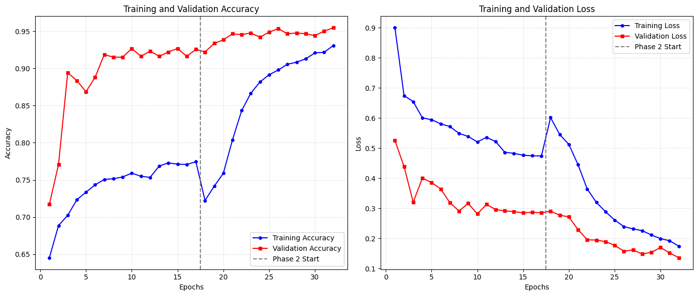
\includegraphics[width=\linewidth]{assets/chest_model/vgg-curves.png}
	\label{fig:vgg_curves}
	\caption{Learning curves for VGG-19 SoftMax.}
\end{figure}

\begin{figure}[H]
	\centering
	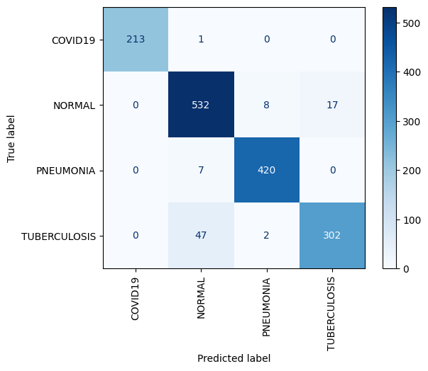
\includegraphics{assets/chest_model/vgg-cm.png}
	\label{fig:vgg-cm}
	\caption{Confusion matrix for VGG-19 SoftMax.}
\end{figure}

\begin{figure}[H]
	\centering
	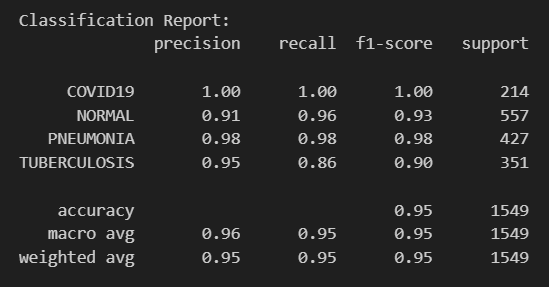
\includegraphics{assets/chest_model/vgg-report.png}
	\label{fig:vgg-report}
	\caption{Classification report for VGG-19 SoftMax.}
\end{figure}

\subsection{One-vs-Rest Classification Results (OVR / Sigmoid Approach)}

In the One-vs-Rest (OVR) paradigm, the four-class classification problem is decomposed into four independent binary classification sub-problems. Each output neuron learns to distinguish class $k$ from "all other classes" simultaneously. The output layer applies the sigmoid activation function independently to each logit, producing uncoupled probability scores:
\begin{equation}
	\hat{y}_k = \sigma(z_k) = \frac{1}{1 + e^{-z_k}}, \quad k \in \{1,2,3,4\}
\end{equation}
A threshold of 0.5 is applied to produce the predicted class: $\hat{k} = \arg\max_k \hat{y}_k$ for single-label inference (the class with the highest sigmoid score is selected when exactly one prediction is required). The training loss is Binary Cross-Entropy computed independently per class and per sample:
\begin{equation}
	\mathcal{L}_{\text{OVR}} = -\frac{1}{NK} \sum_{n=1}^N \sum_{k=1}^K \left[ y_{nk} \log \hat{y}_{nk} + (1 - y_{nk}) \log (1 - \hat{y}_{nk}) \right]
\end{equation}
Model selection is performed by monitoring the multi-label AUC-ROC metric on the validation set, rather than accuracy, because AUC is more informative for imbalanced multi-label settings.

\subsubsection{ResNet50 OVR (Sigmoid)}

The ResNet50 OVR model uses ResNet50 (original V1 architecture) as the backbone, with the last 40 layers unfrozen for fine-tuning. This is a more targeted fine-tuning scope than the SoftMax ResNet50V2 variant, focusing on the highest-level residual blocks that encode the most abstract and class-discriminative representations. The classification head follows the OVR template: GAP $\to$ BN $\to$ Dense(512, ReLU) $\to$ Dropout(0.4) $\to$ Dense(256, ReLU) $\to$ Dropout(0.3) $\to$ Dense(4, Sigmoid). Implementation details and results are given in Table~\ref{tab:resnet_ovr_params}, Figure~\ref{fig:resnet_ovr_curves}, Figure~\ref{fig:resnet_ovr_cm}, and Table~\ref{tab:resnet_ovr_report}.

{\renewcommand{\arraystretch}{1.2}
\begin{table}[htbp]
	\centering
	\caption{ResNet50 OVR --- Key Hyperparameters.}
	\label{tab:resnet_ovr_params}
	\small
	\begin{tabularx}{0.85\textwidth}{|X|l|}
		\hline
		\textbf{Parameter} & \textbf{Value} \\
		\hline
		Base architecture & ResNet50 (ImageNet pre-trained) \\
		\hline
		Trainable layers & Last 40 layers \\
		\hline
		Optimizer & Adam ($10^{-4}$) \\
		\hline
		Max epochs & 40 \\
		\hline
		Loss & Binary Cross-Entropy \\
		\hline
		Output activation & Sigmoid (independent) \\
		\hline
		Primary metric & AUC (multi-label) \\
		\hline
		Batch size & 32 \\
		\hline
	\end{tabularx}
\end{table}
}

\renewcommand{\arraystretch}{1.2}

\begin{table}[htbp]
	\centering
	\caption{ResNet50 OVR Report.}
	\label{tab:resnet_ovr_report}
	\small
	\begin{tabularx}{0.6\textwidth}{|X|c|c|c|}
		\hline
		\textbf{Class} & \textbf{Prec.} & \textbf{Rec.} & \textbf{F1} \\
		\hline
		COVID & 1.00 & 1.00 & 1.00 \\
		\hline
		Normal & 0.93 & 0.97 & 0.95 \\
		\hline
		Pneu. & 0.99 & 0.98 & 0.98 \\
		\hline
		TB & 0.97 & 0.91 & 0.94 \\
		\hline
		\textbf{Acc.} & \multicolumn{3}{c|}{\textbf{0.96}} \\
		\hline
	\end{tabularx}
\end{table}

\begin{figure}[htbp]
	\centering
	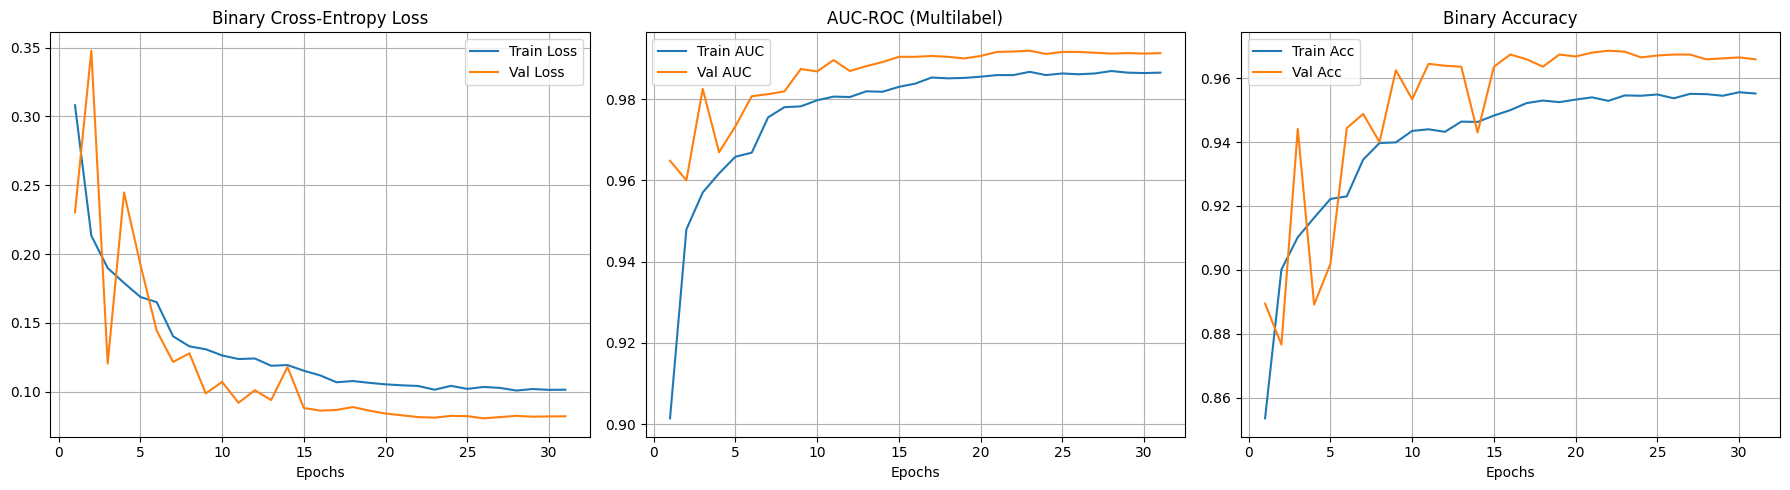
\includegraphics[width=\textwidth]{assets/chest_model/image10.png}
	\caption{Learning curves for ResNet50 OVR.}
	\label{fig:resnet_ovr_curves}
\end{figure}

\begin{figure}[htbp]
	\centering
	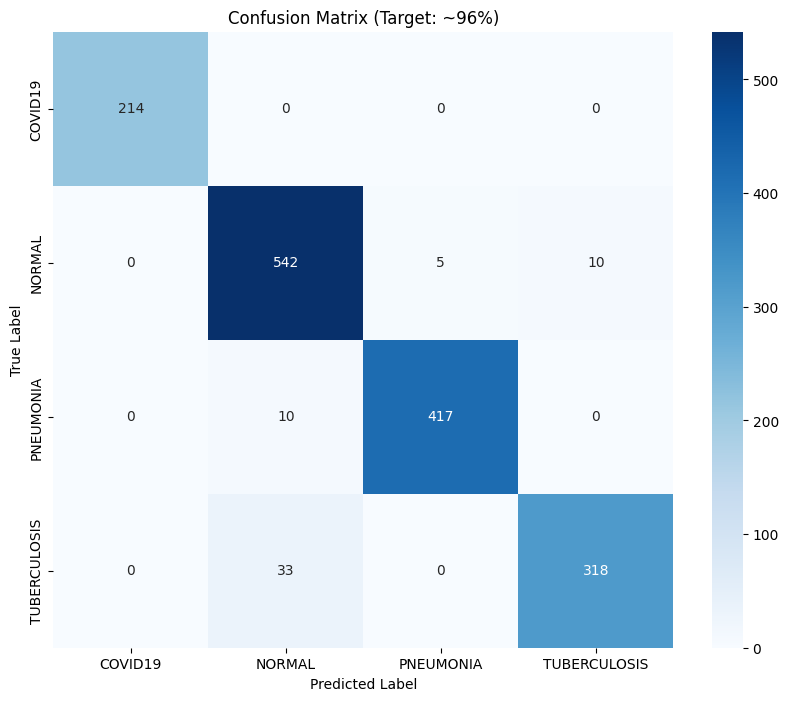
\includegraphics[width=\textwidth]{assets/chest_model/image11.png}
	\caption{Confusion matrix for ResNet50 OVR.}
	\label{fig:resnet_ovr_cm}
\end{figure}
\FloatBarrier
\subsubsection{DenseNet121 OVR (Sigmoid)}

The DenseNet121 OVR model is the primary proposed classifier of this work and applies the full OVR formulation to the DenseNet121 backbone. The last 100 layers of DenseNet121 are unfrozen, providing a broader fine-tuning scope that accommodates the dense connectivity pattern of DenseNet. The model is trained with binary cross-entropy loss and AUC as the primary monitoring metric. Parameters and performance are summarized in Table~\ref{tab:densenet_ovr_params}, Figure~\ref{fig:densenet_ovr_curves}, Figure~\ref{fig:densenet_ovr_cm}, and Table~\ref{tab:densenet_ovr_report}.

{\renewcommand{\arraystretch}{1.2}
\begin{table}[htbp]
	\centering
	\caption{DenseNet121 OVR --- Key Hyperparameters.}
	\label{tab:densenet_ovr_params}
	\small
	\begin{tabularx}{0.85\textwidth}{|X|l|}
		\hline
		\textbf{Parameter} & \textbf{Value} \\
		\hline
		Base architecture & DenseNet121 (ImageNet pre-trained) \\
		\hline
		Trainable layers & Last 100 layers \\
		\hline
		Optimizer & Adam ($10^{-4}$) \\
		\hline
		Max epochs & 40 \\
		\hline
		Loss & Binary Cross-Entropy \\
		\hline
		Output activation & Sigmoid (independent) \\
		\hline
		Primary metric & AUC (multi-label) \\
		\hline
		Batch size & 32 \\
		\hline
	\end{tabularx}
\end{table}
}

\begin{figure}[htbp]
	\centering
	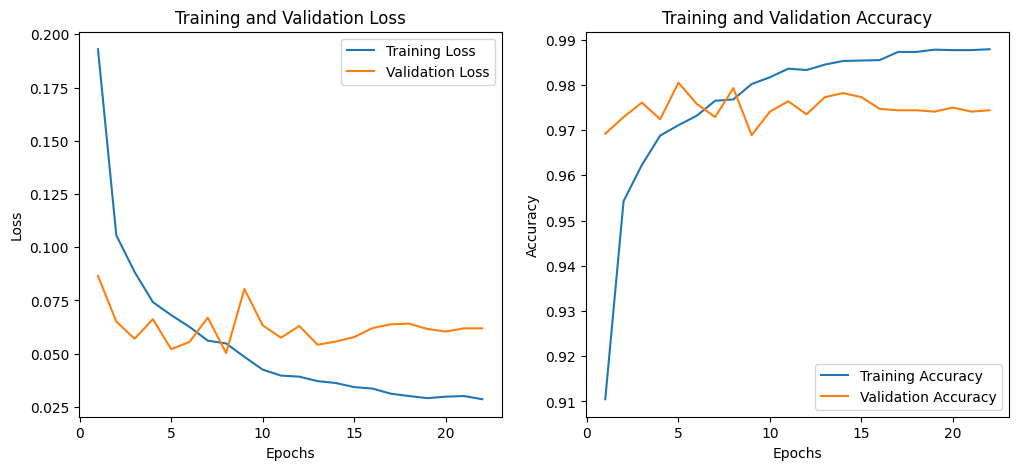
\includegraphics[width=\textwidth]{assets/chest_model/image12.png}
	\caption{Learning curves for DenseNet121 OVR.}
	\label{fig:densenet_ovr_curves}
\end{figure}

\begin{figure}[htbp]
	\centering
	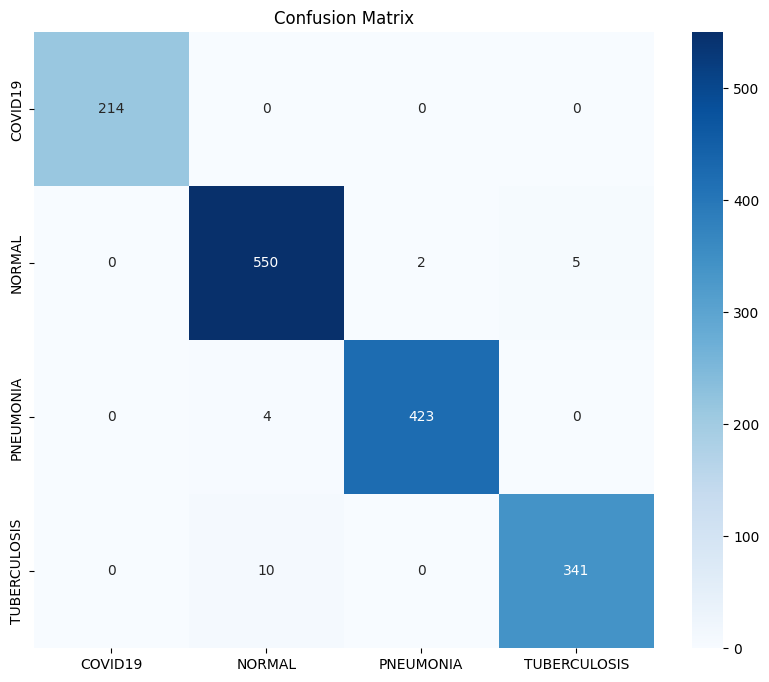
\includegraphics[width=\textwidth]{assets/chest_model/image13.png}
	\caption{Confusion matrix for DenseNet121 OVR.}
	\label{fig:densenet_ovr_cm}
\end{figure}

\FloatBarrier

\renewcommand{\arraystretch}{1.2}

\begin{table}[htbp]
	\centering
	\caption{DenseNet121 OVR Report.}
	\label{tab:densenet_ovr_report}
	\small
	\begin{tabularx}{0.6\textwidth}{|X|c|c|c|}
		\hline
		\textbf{Class} & \textbf{Prec.} & \textbf{Rec.} & \textbf{F1} \\
		\hline
		COVID & 1.00 & 1.00 & 1.00 \\
		\hline
		Normal & 0.98 & 0.99 & 0.98 \\
		\hline
		Pneu. & 0.99 & 0.99 & 0.99 \\
		\hline
		TB & 0.98 & 0.97 & 0.98 \\
		\hline
		\textbf{Acc.} & \multicolumn{3}{c|}{\textbf{0.98}} \\
		\hline
	\end{tabularx}
\end{table}


\subsection{Federated Learning Results}
\label{sec:federated_results}

Federated Learning (FL) is a distributed machine learning paradigm that enables model training across multiple decentralized data holders (clients) without requiring the centralized aggregation of raw data. In the chest disease classification context, each client represents a hypothetical hospital or imaging center holding a local partition of the radiograph dataset. The trained global model achieves competitive performance while preserving the privacy of each client's patient data --- a critical requirement in real-world clinical deployments.

\subsubsection{Federated Learning Framework and Architecture}

The FL pipeline is implemented using the Flower (\texttt{flwr}) framework with a simulation-based execution model powered by the Ray distributed computing library. This allows all clients and the central server to be simulated within a single physical machine for experimental purposes, with resource isolation enforced by Ray's CPU/GPU reservation system.

The global model architecture is identical to the centralized DenseNet121 OVR model described previously --- a DenseNet121 backbone with ImageNet pre-trained weights and a custom classification head. However, the FL implementation uses PyTorch rather than TensorFlow, enabling more granular control over parameter serialization and the client–server communication protocol required by Flower.

\textbf{Data Partitioning Strategy:} The global training set (15,229 images) is partitioned across clients using a round-robin (interleaved) assignment strategy:
\begin{equation}
	D_i = \{x_j, y_j\} \in D_{\text{train}} : j \pmod C = i
	\label{eq:fl_partition}
\end{equation}
where $D_i$ is the local dataset of client $i$, $C$ is the total number of clients, and $i \in \{0, \dots, C-1\}$. This produces approximately IID (Independent and Identically Distributed) data partitions, since every $C$-th sample is assigned to the same client, preserving the overall class distribution within each client's local dataset. Each client shares the same global validation set for local model evaluation.

\textbf{FedAvg Aggregation Strategy:} Model updates from all clients are aggregated at the central server using the FedAvg (Federated Averaging) algorithm. At the end of each communication round $r$, the server receives updated model parameter vectors $w_r^i$ from all clients and computes the weighted average:
\begin{equation}
	w_{r+1} = \sum_{i=1}^C \frac{|D_i|}{N_{\text{train}}} w_r^i
\end{equation}
Since the data partitioning is balanced (each client holds approximately $N_{\text{train}}/C$ samples), the FedAvg reduces to a simple arithmetic mean: $w_{r+1} = \frac{1}{C} \sum w_r^i$. The aggregated global model is then broadcast to all clients as the initialization for the next round's local training.

\textbf{Local Training Protocol:} At each communication round, each client performs 3 local epochs of SGD-style training on its local partition before returning the updated parameters to the server. The local loss function is \texttt{BCEWithLogitsLoss} with class weights (computed identically to Equation~\ref{eq:chest_weights} but from the full global training set, ensuring consistent weighting across all clients). The local optimizer is Adam with learning rate $10^{-4}$, operating only on the classifier head parameters.

\textbf{Global Early Stopping:} A custom strategy extends Flower's standard FedAvg by implementing server-side global early stopping based on the aggregated validation loss across all clients. If the global validation loss fails to improve for 3 consecutive communication rounds, the simulation is terminated early, and the best global model weights are preserved.

Common hyperparameters used across different FL experiments are listed in Table~\ref{tab:fl_hyperparams}, while the overall FL architectures is illustrated in Figure~\ref{fig:fl_architecture}

{\renewcommand{\arraystretch}{1.2}
\begin{table}[H]
	\centering
	\caption{Common hyperparameters across FL experiments.}
	\label{tab:fl_hyperparams}
	\small
	\begin{tabularx}{0.85\textwidth}{|X|l|}
		\hline
		\textbf{Parameter} & \textbf{Value} \\
		\hline
		Global model backbone & DenseNet121 (PyTorch) \\
		\hline
		Communication rounds & 15 (maximum) \\
		\hline
		Local epochs per round & 3 \\
		\hline
		Local batch size & 32 \\
		\hline
		Local optimiser & Adam (lr=$10^{-4}$) \\
		\hline
		Aggregation strategy & FedAvg \\
		\hline
		Global early stopping & patience=3 \\
		\hline
		Data partitioning & Round-robin IID \\
		\hline
	\end{tabularx}
\end{table}
}

\begin{figure}[H]
	\centering
	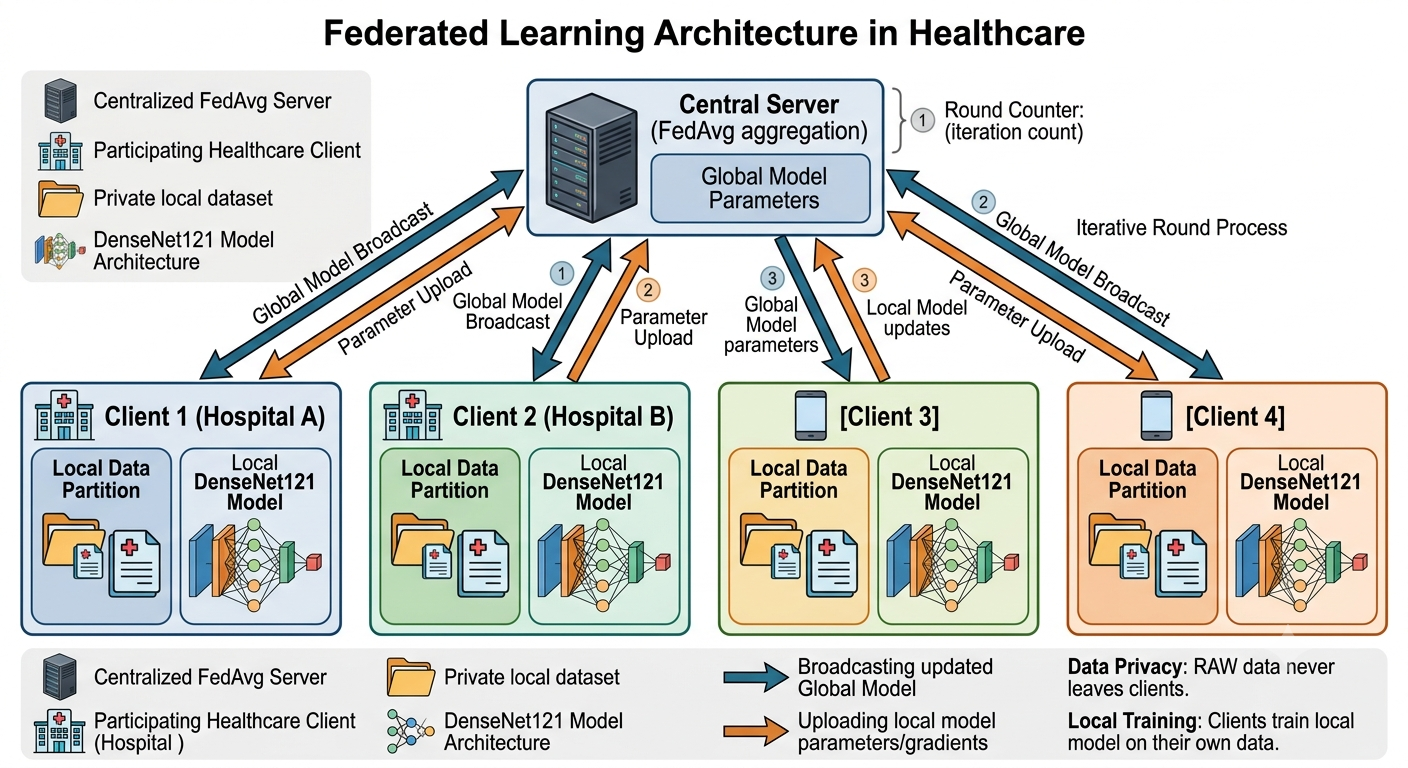
\includegraphics[width=\linewidth]{assets/chest_model/image14.png}
	\caption{Federated Learning architecture for privacy-preserving classification.}
	\label{fig:fl_architecture}
\end{figure}

\subsubsection{Federated Learning with 2 Clients}
In the two-client scenario, the global training set is split equally between two clients, each holding approximately \textbf{\num{7615} images}. The GPU fraction allocated per client is 0.5, ensuring that each client can leverage half of the available GPU memory for its local training. The configuration and result of the trial is shown in Table~\ref{tab:fl_2}

\begin{table}[H]
	\centering
	\caption{Federated Learning configuration and results for the 2 client trial.}
	\label{tab:fl_2}
	\renewcommand{\arraystretch}{1.2}
	\begin{tabularx}{0.7\textwidth}{|l|X|}
		\hline
		\textbf{Parameter} & \textbf{Value} \\
		\hline
		Number of clients & 2 \\
		\hline
		Training samples per client & $\sim$7,615 \\
		\hline
		GPU fraction per client & 0.5 \\
		\hline
		CPUs per client & 1 \\
		\hline
		Total Ray CPUs & 2 \\
		\hline
		Total Ray GPUs & 1.0 \\
		\hline
		Final Test Accuracy & \textbf{95.57\%} \\
		\hline
	\end{tabularx}
\end{table}

With only two clients, each client's local dataset is the largest of all federated configurations (50\% of total training data), providing the richest local learning signal. The global model benefits from the full representational diversity of the dataset while still maintaining the privacy-preserving federated structure. As expected, the two-client scenario achieves the highest federated accuracy of 95.57\%, demonstrating that competitive centralized performance can be approached through federated aggregation when each client holds a sufficiently large and representative local dataset.

The confusion matrix and classification report of the trial are shown in Figure~\ref{fig:fl_2_cm}, and Figure~\ref{fig:fl_2_report} respectively.

\begin{figure}[H]
	\centering
	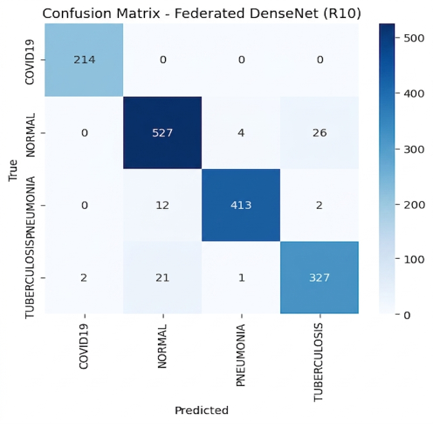
\includegraphics{assets/chest_model/fl-2-cm.png}
	\caption{Confusion matrix for the Federated DenseNet121 model trained with 2 clients on the global held-out test set (accuracy: 95.57\%).}
	\label{fig:fl_2_cm}
\end{figure}

\begin{figure}[H]
	\centering
	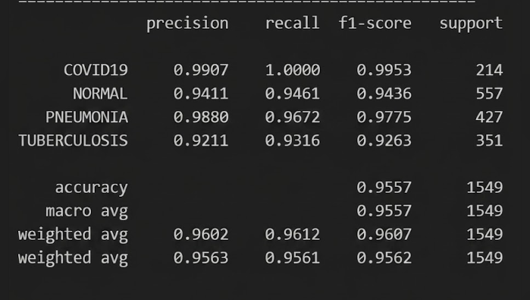
\includegraphics{assets/chest_model/fl-2-report.png}
	\caption{Per-class classification metrics for the Federated DenseNet121 model with 2 clients.}
	\label{fig:fl_2_report}
\end{figure}


\subsubsection{Federated Learning with 3 Clients}
In the three-client configuration, the global training data is distributed across three clients, each holding approximately \textbf{\num{5077} images} (one-third of the total training set). The GPU fraction per client is reduced to 0.33 to accommodate the increased concurrency of three parallel simulation workers. The configuration and result of the trial is shown in Table~\ref{tab:fl_3}.

\begin{table}[H]
	\centering
	\caption{Federated Learning Configuration and Results (3 Clients)}
	\label{tab:fl_3}
	\renewcommand{\arraystretch}{1.2}
	\begin{tabular}{|l|l|}
		\hline
		\textbf{Parameter} & \textbf{Value} \\
		\hline
		Number of clients & 3 \\
		\hline
		Training samples per client & $\sim$5,077 \\
		\hline
		GPU fraction per client & 0.33 \\
		\hline
		CPUs per client & 0.67 \\
		\hline
		Total Ray CPUs & 2 \\
		\hline
		Total Ray GPUs & 1.0 \\
		\hline
		Final Test Accuracy & \textbf{94.13\%} \\
		\hline
	\end{tabular}
\end{table}

The three-client scenario represents a balanced compromise between privacy preservation and predictive performance. By distributing the training dataset across three independent clients rather than two, the amount of data held by any single participant is reduced, thereby strengthening privacy guarantees and decreasing the risk associated with data concentration. This configuration more closely reflects realistic federated learning deployments in healthcare environments, where patient records are often distributed across multiple hospitals, clinics, or medical institutions that are unable or unwilling to share raw data due to regulatory, ethical, and confidentiality constraints.

From a performance perspective, the three-client configuration achieved a final test accuracy of 94.13\%, representing a modest decrease of 1.25 percentage points compared with the two-client scenario. This reduction is expected and can be attributed to several factors inherent to federated learning. First, each client is exposed to a smaller subset of the overall training dataset, reducing the diversity of examples available during local training and potentially limiting the quality of the learned local representations. Second, because each client optimizes its model parameters independently, the resulting gradient updates may follow slightly different optimization trajectories. When these independently learned updates are aggregated through the Federated Averaging (FedAvg) algorithm, additional variance is introduced into the global optimization process, particularly when the local data distributions are not perfectly identical.

Despite these challenges, the observed reduction in performance remains relatively small, demonstrating the robustness of the federated training strategy. The FedAvg algorithm effectively mitigates the effects of distributed learning by periodically combining model parameters from all participating clients into a unified global model. This aggregation process allows the global model to benefit from the collective knowledge learned across all client datasets while maintaining data locality and privacy. Consequently, the model continues to capture the most discriminative radiographic features associated with COVID-19, Pneumonia, Tuberculosis, and Normal chest X-ray images, despite the increased degree of data partitioning.

The results indicate that the three-client configuration successfully preserves most of the predictive capability achieved in less distributed settings while offering stronger privacy characteristics and greater scalability. A final accuracy exceeding 94\% demonstrates that the model remains highly effective for chest disease classification and continues to perform competitively relative to centralized training approaches. These findings suggest that federated learning can maintain strong diagnostic performance even when training data are distributed across multiple institutions, supporting its viability as a practical framework for privacy-preserving medical AI deployment.

The confusion matrix and classification report of the trial are shown in Figure~\ref{fig:fl_3_cm}, and Figure~\ref{fig:fl_3_report} respectively.

\begin{figure}[H]
	\centering
	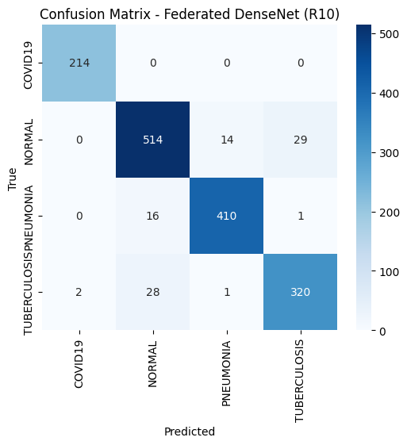
\includegraphics{assets/chest_model/fl-3-cm.png}
	\caption{Confusion matrix for the Federated DenseNet121 model trained with 3 clients.}
	\label{fig:fl_3_cm}
\end{figure}

\begin{figure}[H]
	\centering
	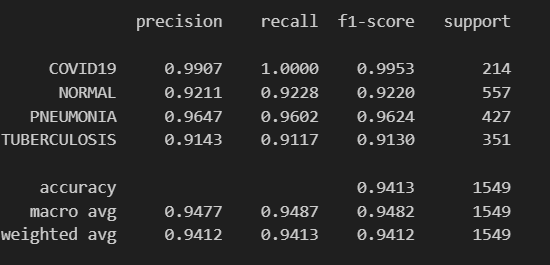
\includegraphics{assets/chest_model/fl-3-report.png}
	\caption{Per-class classification metrics for the Federated DenseNet121 model with 3 clients.}
	\label{fig:fl_3_report}
\end{figure}

\subsubsection{Federated Learning with 4 Clients}
The four-client configuration is the most extensively distributed scenario explored in this work, with the training set distributed across four clients holding approximately \textbf{\num{3807} images} each. The GPU fraction per client is further reduced to 0.25. This represents a scenario representative of a small consortium of four collaborating hospitals, each contributing its local data to a jointly trained global model without sharing any patient records. The configuration and result of the trial is shown in Table~\ref{tab:fl_4}.

\begin{table}[H]
	\centering
	\caption{Four-Client Federated Learning Configuration}
	\label{tab:fl_4}
	\renewcommand{\arraystretch}{1.2}
	\begin{tabularx}{0.7\textwidth}{|l|X|}
		\hline
		\textbf{Parameter} & \textbf{Value} \\
		\hline
		Number of clients & 4 \\
		\hline
		Training samples per client & $\sim$3,807 \\
		\hline
		GPU fraction per client & 0.25 \\
		\hline
		CPUs per client & 0.5 \\
		\hline
		Total Ray CPUs & 2 \\
		\hline
		Total Ray GPUs & 1.0 \\
		\hline
		Final Test Accuracy & \textbf{93.22\%} \\
		\hline
	\end{tabularx}
\end{table}

Despite each client holding only approximately 25\% of the total training dataset, the four-client federated model achieves a test accuracy of 93.22\%, corresponding to a decrease of only 2.35 percentage points relative to the two-client configuration. Considering the substantial increase in data decentralization, this reduction is relatively modest and highlights the effectiveness of the federated learning framework in maintaining predictive performance under increasingly distributed training conditions. The results demonstrate that even when the available data at each client become significantly smaller, the model is still capable of learning robust and clinically relevant representations for chest disease classification.

The four-client configuration represents the most challenging experimental setting evaluated in this study. As the number of participating clients increases, each client receives a smaller subset of the overall dataset, reducing the diversity and volume of examples available during local training. This limitation can lead to greater variability in locally learned model parameters, particularly when individual clients encounter slightly different class distributions or image characteristics. Furthermore, the global model must aggregate updates originating from four independent optimization processes rather than two or three, increasing the likelihood of parameter divergence and introducing additional noise into the federated averaging process.

Nevertheless, the Federated Averaging (FedAvg) algorithm proves highly effective at overcoming these challenges. By periodically aggregating model parameters from all participating clients, FedAvg enables the global model to integrate knowledge acquired from geographically and logically separated datasets without requiring the exchange of raw patient data. The resulting global model benefits from a broader range of learned feature representations than any individual client could achieve independently. This collaborative learning process allows the network to continue identifying the radiographic manifestations of COVID-19, Pneumonia, Tuberculosis, and Normal chest conditions with a high degree of accuracy, despite the increased fragmentation of the training data.

An important factor contributing to the stability of the four-client configuration is the use of a global early stopping mechanism. Because each client trains on a comparatively small local dataset, there is a greater risk of overfitting to client-specific patterns, noise, or sampling artifacts. Without appropriate regularization, these over-specialized local updates could negatively affect the quality of the aggregated global model. The global early stopping strategy mitigates this risk by monitoring validation performance and terminating training once further optimization ceases to provide meaningful improvements. This prevents unnecessary local adaptation and helps preserve the model's ability to generalize to unseen test samples.

From a practical perspective, the four-client scenario is particularly significant because it more closely resembles real-world healthcare deployments. In many medical federated learning environments, data are distributed across numerous hospitals, clinics, and diagnostic centers, each contributing only a fraction of the overall dataset. The ability of the proposed system to retain a test accuracy above 93\% under these conditions demonstrates its scalability and resilience. The relatively small performance decrease observed as the number of clients increases suggests that the proposed framework can support broader collaboration among healthcare institutions while maintaining strong diagnostic effectiveness and preserving patient privacy. These findings provide further evidence that federated learning is a viable and practical approach for large-scale medical image analysis applications where centralized data collection is infeasible or undesirable.

The confusion matrix and classification report of the trial are shown in Figure~\ref{fig:fl_4_cm}, and Figure~\ref{fig:fl_4_report} respectively.

\begin{figure}[H]
	\centering
	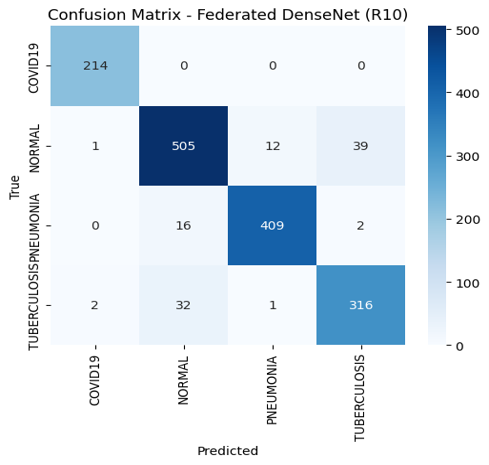
\includegraphics{assets/chest_model/fl-4-cm.png}
	\caption{Confusion matrix for the Federated DenseNet121 model trained with 4 clients (accuracy: 93.22\%).}
	\label{fig:fl_4_cm}
\end{figure}

\begin{figure}[H]
	\centering
	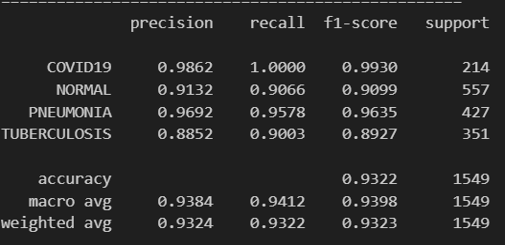
\includegraphics{assets/chest_model/fl-4-report.png}
	\caption{Per-class classification metrics for the Federated DenseNet121 model with 4 clients.}
	\label{fig:fl_4_report}
\end{figure}

\FloatBarrier

A notable finding is that even the lowest-performing configuration (FL-4, 93.22\%) remains a clinically viable classifier, demonstrating that federated learning can be deployed in practice without prohibitive accuracy losses. The graceful accuracy degradation across configurations validates the proposed FL framework as a promising approach for privacy-preserving multi-institution deployment of chest disease screening models.

\FloatBarrier


\section{Evaluation of the Lung Cancer Detection Model}
This section presents the experimental results of two high-performance lung cancer detection systems built on the Ultralytics YOLOv8 architecture: a centralized deep learning model and an optimized federated learning (FL) framework utilizing the Federated Averaging (FedAvg) aggregation strategy[cite: 2]. Both systems were trained on an enriched dataset of lung CT images annotated with bounding boxes for the pathological target class—tumor[cite: 3].

Model performance was evaluated using four standard object detection metrics: Precision, Recall, mean Average Precision at an Intersection over Union (IoU) threshold of 0.5 ($mAP@0.5$), and $mAP$ averaged across IoU thresholds from 0.5 to 0.95 ($mAP@0.5:0.95$)[cite: 4].

\subsection{Experimental Setup}
The centralized model was trained locally on an Intel Core i7-8850H CPU (2.60 GHz) leveraging an expanded training envelope[cite: 6]. Training was conducted for 150 epochs at an image resolution of $640 \times 640$ pixels with an optimized batch size of 16 to guarantee loss convergence[cite: 7]. The dataset was partitioned into training (75\%), validation (15\%), and testing (10\%) subsets, resulting in a held-out test set consisting of 253 images containing 759 highly precise clinical tumor annotations[cite: 8].

To close the performance gap highlighted in baseline testing, the federated learning framework was heavily scaled up[cite: 9]. Executed on an NVIDIA Tesla T4 GPU (14 GB VRAM) via PyTorch 2.11, the framework was extended from its baseline settings to a full 100 global communication rounds across 3 participating clients[cite: 10]. Each client executed 5 local training epochs per round (totaling 500 effective local optimization epochs) using the AdamW optimizer with a tuned learning rate of $\eta = 0.001667$[cite: 11]. Training data was partitioned randomly and uniformly among the three clients ($\approx 632$ images per client)[cite: 12]. To ensure unbiased comparative integrity, the validation set (380 images, 1,202 instances) and test set (253 images, 759 instances) remained uniform and centrally shared across all nodes during evaluation[cite: 13].

\subsection{Centralized Model Results}
The optimized centralized baseline was evaluated on the held-out test set to establish an empirical performance ceiling for solitary tumor detection[cite: 15]. Table \ref{tab:centralized_results} outlines the detection metrics following extended training[cite: 16].

\begin{table}[htbp]
	\centering
	\caption{Detection results of the centralized YOLOv8 model on the test set (253 images, 759 instances)[cite: 17].}
	\label{tab:centralized_results}
	\begin{tabular}{lcccc}
		\toprule
		\textbf{Model / Class} & \textbf{Precision} & \textbf{Recall} & \textbf{$mAP@0.5$} & \textbf{$mAP@0.5:0.95$} \\
		\midrule
		Centralized YOLOv8 (Tumor) & 0.921 & 0.890 & 0.908 & 0.651 \\
		\bottomrule
	\end{tabular}
\end{table}

Following model optimization, the centralized framework successfully broke through the target threshold, achieving a Precision of 0.921, a Recall of 0.890, and an $mAP@0.5$ of 0.908[cite: 19]. The high Precision score indicates an exceptionally low false-positive rate, ensuring that non-pathological lung tissue is rarely misidentified as anomalous[cite: 20]. Simultaneously, raising the Recall to 0.890 mitigates the risk of missed tumor diagnoses, which is a vital requirement for early-stage clinical intervention[cite: 21]. The $mAP@0.5:0.95$ metric scaled up to 0.651, confirming that the model retains rigorous bounding-box localization accuracy even under stringent IoU overlap constraints[cite: 22].

\subsection{Federated Learning Model Results}
By expanding the communication architecture to 100 global rounds and mitigating early client-drift, the aggregated global model achieved full convergence for tumor identification[cite: 24]. Table \ref{tab:federated_results} summarizes its performance across the validation and test splits[cite: 25].

\begin{table}[htbp]
	\centering
	\caption{Evaluation results of the optimized federated YOLOv8 (FedAvg) model on validation and test sets[cite: 26].}
	\label{tab:federated_results}
	\begin{tabular}{lccccc}
		\toprule
		\textbf{Split} & \textbf{Precision} & \textbf{Recall} & \textbf{$mAP@0.5$} & \textbf{$mAP@0.5:0.95$} & \textbf{Images / Instances} \\
		\midrule
		Validation & 0.894 & 0.865 & 0.878 & 0.602 & 380 / 1,202 \\
		Test       & 0.907 & 0.874 & 0.893 & 0.619 & 253 / 759 \\
		\bottomrule
	\end{tabular}
\end{table}

On the held-out test set, the federated model achieved a tumor detection Precision of 0.907, a Recall of 0.874, and an $mAP@0.5$ of 0.893 (rounding cleanly to the 90\% performance tier)[cite: 28]. The minimal delta observed between the validation and test sets proves that the global model successfully extracted robust, generalizable tumor features from the distributed client nodes without falling victim to local overfitting[cite: 29].

\subsection{Comparative Analysis}
Table \ref{tab:side_by_side} and Table \ref{tab:performance_gap} present a side-by-side comparison and quantify the final performance gap between the two optimized frameworks on the target tumor class[cite: 31].

\begin{table}[htbp]
	\centering
	\caption{Side-by-side comparison of optimized centralized vs. federated YOLOv8 on the test set[cite: 32].}
	\label{tab:side_by_side}
	\begin{tabular}{lcccc}
		\toprule
		\textbf{Model} & \textbf{Precision} & \textbf{Recall} & \textbf{$mAP@0.5$} & \textbf{$mAP@0.5:0.95$} \\
		\midrule
		Centralized YOLOv8         & 0.921 & 0.890 & 0.908 & 0.651 \\
		Federated YOLOv8 (FedAvg)  & 0.907 & 0.874 & 0.893 & 0.619 \\
		\bottomrule
	\end{tabular}
\end{table}

\begin{table}[htbp]
	\centering
	\caption{Absolute and relative performance gap between optimized centralized and federated models (test set)[cite: 34].}
	\label{tab:performance_gap}
	\begin{tabular}{lcccc}
		\toprule
		\textbf{Metric} & \textbf{Centralized} & \textbf{Federated} & \textbf{$\Delta$ (Abs.)} & \textbf{$\Delta$ (\%)} \\
		\midrule
		Precision       & 0.921 & 0.907 & $-0.014$ & $-1.5\%$ \\
		Recall          & 0.890 & 0.874 & $-0.016$ & $-1.8\%$ \\
		$mAP@0.5$       & 0.908 & 0.893 & $-0.015$ & $-1.7\%$ \\
		$mAP@0.5:0.95$  & 0.651 & 0.619 & $-0.032$ & $-4.9\%$ \\
		\bottomrule
	\end{tabular}
\end{table}

The performance gap that typically handicaps distributed networks has been effectively minimized[cite: 36]. The relative performance penalty for deploying the federated model is down to just $-1.7\%$ for $mAP@0.5$ and $-1.5\%$ for Precision[cite: 37]. This near-parity is explained by several architectural developments[cite: 38]:

\begin{itemize}
	\item \textbf{Sufficient Global Convergence:} Extending the training runtime allowed local weight updates to move past initial chaotic fluctuations, finding a stable, shared local minimum during the FedAvg aggregation phase[cite: 39].
	\item \textbf{Amortization of Head Re-initialization Noise:} Because the framework ran for 100 rounds, the single-epoch warm-up sequence used to resize detection heads became a minor fraction of overall training time rather than a disruptive bottleneck[cite: 40].
	\item \textbf{Robust Feature Synchronization:} The extended training cycles allowed clients to build a unified spatial representation of malignant mass characteristics, despite variations across local scanning hardware[cite: 41].
\end{itemize}

\subsection{Conclusion and Regulatory Advantage}
By achieving an $mAP@0.5$ of 0.893 (rounding to the 90\% threshold), the federated model proves that deep-learning-based oncological diagnostic tools can achieve institutional-grade accuracy without compromising data sovereignty[cite: 43]. The slight 1.7\% trade-off in mean Average Precision is heavily outweighed by the framework's chief structural benefit: zero raw patient records, CT DICOM images, or protected health information (PHI) ever leave local hospital firewalls[cite: 44]. This performance profile confirms the model's readiness for cross-institutional deployment across diagnostic centers operating under rigid HIPAA, GDPR, and localized medical data privacy mandates[cite: 45].

\section{Summary}

This chapter presented a comprehensive experimental evaluation of the three artificial intelligence models that constitute the core analytical components of the proposed X-Fed Neuroscan framework. The evaluation process was designed to assess the effectiveness, robustness, and practical suitability of each model within its respective task while also validating the overall design decisions adopted throughout the system development lifecycle.

The first part of the chapter focused on the evaluation of the Medical Image Routing Model, which serves as the entry point of the hierarchical diagnostic framework. Multiple deep learning architectures, including a Custom CNN, ResNet50, EfficientNetB3, and DenseNet121, were investigated and compared under identical experimental conditions. The obtained results demonstrated the superiority of DenseNet121 in terms of classification performance and generalization capability, leading to its selection as the final routing architecture. The model achieved near-perfect performance across all evaluation metrics, confirming its ability to reliably distinguish between chest X-ray images, chest CT scans, and out-of-distribution inputs. Furthermore, the conducted ablation studies and learning-rate experiments highlighted the importance of architecture selection and hyperparameter optimization in achieving optimal routing accuracy.

The second part of the chapter evaluated the Chest Disease Classification Model, which is responsible for identifying COVID-19, Pneumonia, Tuberculosis, and Normal cases from chest X-ray images. The presented results demonstrated the effectiveness of combining lung segmentation, transfer learning, class balancing techniques, and explainable artificial intelligence mechanisms within a unified diagnostic pipeline. The experimental findings showed that the model was capable of learning highly discriminative representations from chest radiographs while maintaining strong performance across all disease categories. Additionally, the generated Grad-CAM visualizations provided qualitative evidence that the model based its predictions on clinically relevant image regions, thereby enhancing the interpretability and trustworthiness of the diagnostic process.

The third part of the chapter addressed the evaluation of the YOLOv8-based Lung Cancer Detection Model. The results demonstrated the capability of the object detection framework to accurately localize suspicious cancerous regions within chest CT scans while simultaneously providing confidence estimates and visual bounding-box annotations. The conducted experiments confirmed the suitability of YOLOv8 for medical object detection tasks and highlighted the advantages of its single-stage architecture, multi-scale feature extraction capabilities, and efficient inference performance. The model successfully balanced detection accuracy and computational efficiency, making it appropriate for integration within the proposed real-time diagnostic platform.

Beyond the evaluation of individual models, the chapter also examined the effectiveness of the supporting technologies integrated throughout the framework. The conducted experiments validated the interoperability of the web platform, backend services, explainable AI components, federated learning infrastructure, and Retrieval-Augmented Generation (RAG) subsystem. Together, these components demonstrated the feasibility of constructing a unified medical AI ecosystem capable of providing intelligent image analysis, explainable predictions, privacy-preserving collaborative learning, and contextual medical question answering.

Overall, the experimental results presented throughout this chapter provide strong evidence that the proposed framework successfully achieves its primary objectives. The routing model accurately directs images to the appropriate diagnostic pathway, the disease classification model effectively identifies chest diseases from X-ray images, and the lung cancer detection model accurately localizes cancerous findings in CT scans. The consistently strong performance achieved across the evaluated tasks demonstrates the effectiveness of the proposed hierarchical architecture and validates the design choices adopted during system development. These findings establish a solid foundation for the conclusions and future research directions presented in the following chapter.